\documentclass[aspectratio=169]{beamer}

% Minimal theme
\usetheme{default}
\usecolortheme{dove}

% Remove navigation symbols
\setbeamertemplate{navigation symbols}{}
\setbeamertemplate{footline}{%
  \hfill{\large\insertframenumber\,/\,\inserttotalframenumber}\hspace{0.8em}\vspace{0.5em}%
}

% Colors
\definecolor{popblue}{RGB}{52, 101, 164}
\definecolor{sampred}{RGB}{204, 0, 0}
\definecolor{paramgreen}{RGB}{0, 140, 70}
\definecolor{lightbg}{RGB}{245, 245, 250}
\definecolor{warnred}{RGB}{180, 40, 40}
\definecolor{orange1}{RGB}{220, 120, 0}
\definecolor{violet1}{RGB}{120, 50, 160}

\setbeamercolor{frametitle}{fg=popblue}
\setbeamercolor{title}{fg=popblue}

% Packages
\usepackage{pgfplots}
\usepackage{tikz}
\usetikzlibrary{shapes, arrows.meta, positioning, calc, decorations.pathreplacing, patterns}
\pgfplotsset{compat=1.18}
\usepackage{amsmath, amssymb}
\usepackage{array}
\usepackage{fontenc}

\title{Inference Optimization}
\subtitle{KV-Cache $\cdot$ Flash Attention $\cdot$ Quantization $\cdot$ Distillation $\cdot$ Speculative Decoding}
\date{}

\begin{document}

% ============================================================
% TITLE
% ============================================================
\begin{frame}
\titlepage
\end{frame}

% ============================================================
% THE INFERENCE CHALLENGE
% ============================================================
\begin{frame}
\frametitle{The inference challenge}

\begin{center}
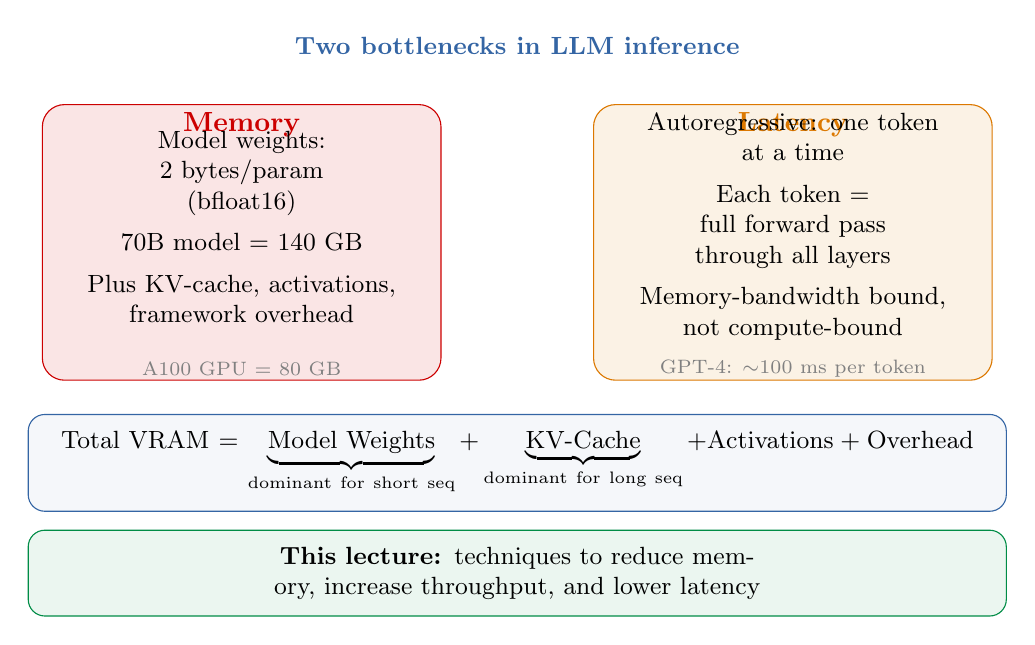
\begin{tikzpicture}
  % Two bottlenecks
  \node[font=\small\bfseries, text=popblue] at (0, 3.5) {Two bottlenecks in LLM inference};

  % Memory
  \node[draw=sampred, fill=sampred!10, rounded corners=8pt, minimum width=5cm, minimum height=3.5cm, text width=4.5cm, align=center, inner sep=8pt] at (-3.5, 1) {};
  \node[font=\normalsize\bfseries, text=sampred] at (-3.5, 2.5) {Memory};
  \node[font=\small, text width=4.2cm, align=center] at (-3.5, 1.2) {
    Model weights: 2 bytes/param\\(bfloat16)\\[4pt]
    70B model $=$ 140 GB\\[4pt]
    Plus KV-cache, activations,\\framework overhead
  };
  \node[font=\scriptsize, text=gray] at (-3.5, -0.6) {A100 GPU = 80 GB};

  % Latency
  \node[draw=orange1, fill=orange1!10, rounded corners=8pt, minimum width=5cm, minimum height=3.5cm, text width=4.5cm, align=center, inner sep=8pt] at (3.5, 1) {};
  \node[font=\normalsize\bfseries, text=orange1] at (3.5, 2.5) {Latency};
  \node[font=\small, text width=4.2cm, align=center] at (3.5, 1.2) {
    Autoregressive: one token\\at a time\\[4pt]
    Each token = full forward pass\\through all layers\\[4pt]
    Memory-bandwidth bound,\\not compute-bound
  };
  \node[font=\scriptsize, text=gray] at (3.5, -0.6) {GPT-4: $\sim$100 ms per token};

  % Total inference memory formula
  \node[draw=popblue, fill=popblue!5, rounded corners=6pt, text width=12cm, align=center, inner sep=6pt, font=\small] at (0, -1.8) {
    $\text{Total VRAM} = \underbrace{\text{Model Weights}}_{\text{dominant for short seq}} + \underbrace{\text{KV-Cache}}_{\text{dominant for long seq}} + \text{Activations} + \text{Overhead}$
  };

  % What we'll cover
  \node[draw=paramgreen, fill=paramgreen!8, rounded corners=6pt, text width=12cm, align=center, inner sep=6pt, font=\small] at (0, -3.2) {
    \textbf{This lecture:} techniques to reduce memory, increase throughput, and lower latency
  };
\end{tikzpicture}
\end{center}
\end{frame}

% ============================================================
% MEMORY ARITHMETIC
% ============================================================
\begin{frame}
\frametitle{Memory arithmetic}

\begin{center}
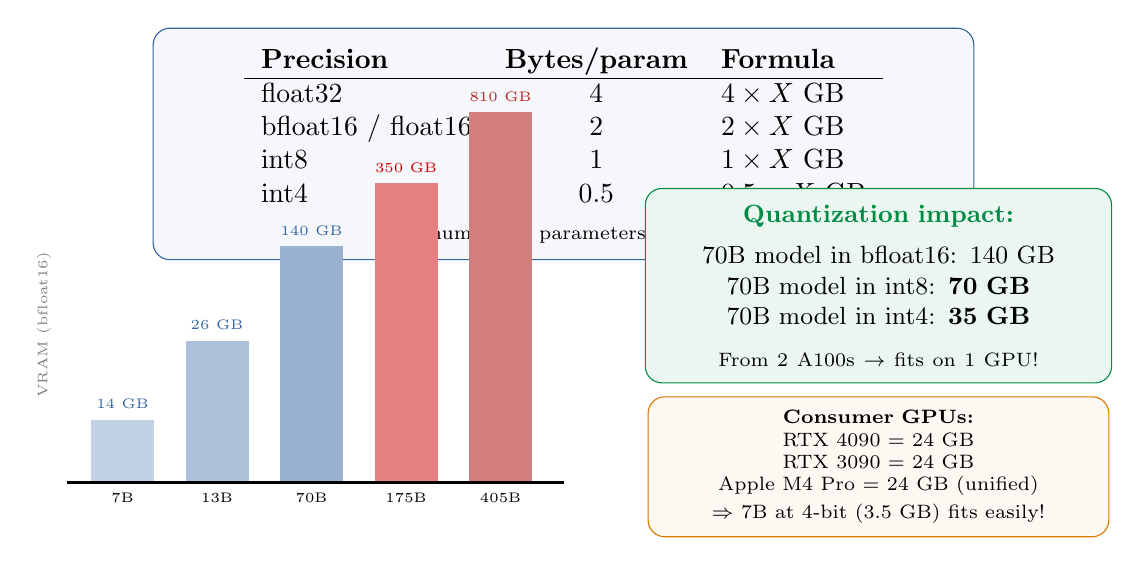
\begin{tikzpicture}
  % Rules of thumb
  \node[font=\small\bfseries, text=popblue] at (0, 3.5) {How much VRAM for the model weights alone?};

  % Precision table
  \node[draw=popblue, fill=popblue!5, rounded corners=6pt, text width=10cm, align=center, inner sep=6pt] at (0, 2.3) {
    \begin{tabular}{l c l}
      \textbf{Precision} & \textbf{Bytes/param} & \textbf{Formula} \\
      \hline
      float32 & 4 & $4 \times X$ GB \\
      bfloat16 / float16 & 2 & $2 \times X$ GB \\
      int8 & 1 & $1 \times X$ GB \\
      int4 & 0.5 & $0.5 \times X$ GB \\
    \end{tabular}\\[4pt]
    {\scriptsize $X$ = number of parameters in billions}
  };

  % Bar chart
  \fill[popblue!30] (-6, -2) rectangle (-5.2, -1.2);
  \node[font=\tiny] at (-5.6, -2.2) {7B};
  \node[font=\tiny, text=popblue] at (-5.6, -1) {14 GB};

  \fill[popblue!40] (-4.8, -2) rectangle (-4, -0.2);
  \node[font=\tiny] at (-4.4, -2.2) {13B};
  \node[font=\tiny, text=popblue] at (-4.4, 0) {26 GB};

  \fill[popblue!50] (-3.6, -2) rectangle (-2.8, 1);
  \node[font=\tiny] at (-3.2, -2.2) {70B};
  \node[font=\tiny, text=popblue] at (-3.2, 1.2) {140 GB};

  \fill[sampred!50] (-2.4, -2) rectangle (-1.6, 1.8);
  \node[font=\tiny] at (-2, -2.2) {175B};
  \node[font=\tiny, text=sampred] at (-2, 2) {350 GB};

  \fill[warnred!60] (-1.2, -2) rectangle (-0.4, 2.7);
  \node[font=\tiny] at (-0.8, -2.2) {405B};
  \node[font=\tiny, text=warnred] at (-0.8, 2.9) {810 GB};

  % Axis
  \draw[thick] (-6.3, -2) -- (0, -2);
  \node[font=\tiny, text=gray, rotate=90] at (-6.6, 0) {VRAM (bfloat16)};

  % Quantization impact
  \node[draw=paramgreen, fill=paramgreen!8, rounded corners=6pt, text width=5.5cm, align=center, inner sep=6pt, font=\small] at (4, 0.5) {
    \textbf{\textcolor{paramgreen}{Quantization impact:}}\\[4pt]
    70B model in bfloat16: 140 GB\\
    70B model in int8: \textbf{70 GB}\\
    70B model in int4: \textbf{35 GB}\\[4pt]
    {\scriptsize From 2 A100s $\to$ fits on 1 GPU!}
  };

  % Consumer GPU note
  \node[draw=orange1, fill=orange1!5, rounded corners=6pt, text width=5.5cm, align=center, inner sep=5pt, font=\scriptsize] at (4, -1.8) {
    \textbf{Consumer GPUs:}\\
    RTX 4090 = 24 GB\\
    RTX 3090 = 24 GB\\
    Apple M4 Pro = 24 GB (unified)\\[2pt]
    $\Rightarrow$ 7B at 4-bit (3.5 GB) fits easily!
  };
\end{tikzpicture}
\end{center}
\end{frame}

% ============================================================
% PART I HEADER
% ============================================================
\begin{frame}
\begin{center}
\vspace{1.5cm}
{\Huge \textcolor{popblue}{Part I}}

\vspace{0.5cm}
{\Large Attention Optimization}

\vspace{0.5cm}
{\normalsize KV-Cache, MQA/GQA, Flash Attention}
\end{center}
\end{frame}

% ============================================================
% KV-CACHE: THE PROBLEM
% ============================================================
\begin{frame}
\frametitle{KV-Cache --- the redundancy problem}

\begin{center}
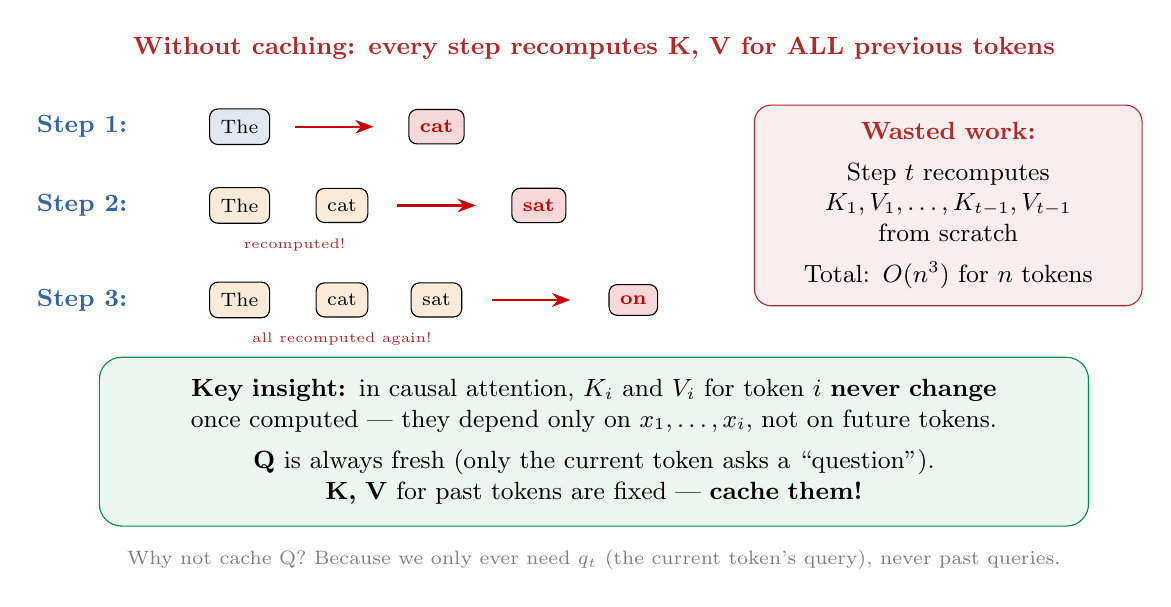
\begin{tikzpicture}
  \node[font=\small\bfseries, text=warnred] at (0, 3.5) {Without caching: every step recomputes K, V for ALL previous tokens};

  % Step 1
  \node[font=\small\bfseries, text=popblue] at (-6.5, 2.5) {Step 1:};
  \node[draw, rounded corners=3pt, fill=popblue!15, inner sep=4pt, font=\scriptsize] at (-4.5, 2.5) {The};
  \draw[-Stealth, thick, sampred] (-3.8, 2.5) -- (-2.8, 2.5);
  \node[draw, rounded corners=3pt, fill=sampred!15, inner sep=4pt, font=\scriptsize\bfseries, text=sampred] at (-2, 2.5) {cat};

  % Step 2
  \node[font=\small\bfseries, text=popblue] at (-6.5, 1.5) {Step 2:};
  \node[draw, rounded corners=3pt, fill=orange1!15, inner sep=4pt, font=\scriptsize] at (-4.5, 1.5) {The};
  \node[draw, rounded corners=3pt, fill=orange1!15, inner sep=4pt, font=\scriptsize] at (-3.2, 1.5) {cat};
  \draw[-Stealth, thick, sampred] (-2.5, 1.5) -- (-1.5, 1.5);
  \node[draw, rounded corners=3pt, fill=sampred!15, inner sep=4pt, font=\scriptsize\bfseries, text=sampred] at (-0.7, 1.5) {sat};
  \node[font=\tiny, text=warnred] at (-3.8, 1.0) {recomputed!};

  % Step 3
  \node[font=\small\bfseries, text=popblue] at (-6.5, 0.3) {Step 3:};
  \node[draw, rounded corners=3pt, fill=orange1!15, inner sep=4pt, font=\scriptsize] at (-4.5, 0.3) {The};
  \node[draw, rounded corners=3pt, fill=orange1!15, inner sep=4pt, font=\scriptsize] at (-3.2, 0.3) {cat};
  \node[draw, rounded corners=3pt, fill=orange1!15, inner sep=4pt, font=\scriptsize] at (-2, 0.3) {sat};
  \draw[-Stealth, thick, sampred] (-1.3, 0.3) -- (-0.3, 0.3);
  \node[draw, rounded corners=3pt, fill=sampred!15, inner sep=4pt, font=\scriptsize\bfseries, text=sampred] at (0.5, 0.3) {on};
  \node[font=\tiny, text=warnred] at (-3.2, -0.2) {all recomputed again!};

  % Complexity
  \node[draw=warnred, fill=warnred!8, rounded corners=6pt, text width=4.5cm, align=center, inner sep=6pt, font=\small] at (4.5, 1.5) {
    \textbf{\textcolor{warnred}{Wasted work:}}\\[4pt]
    Step $t$ recomputes\\$K_1, V_1, \ldots, K_{t-1}, V_{t-1}$\\from scratch\\[4pt]
    Total: $O(n^3)$ for $n$ tokens
  };

  % Key insight
  \node[draw=paramgreen, fill=paramgreen!8, rounded corners=8pt, text width=12cm, align=center, inner sep=8pt, font=\small] at (0, -1.5) {
    \textbf{Key insight:} in causal attention, $K_i$ and $V_i$ for token $i$ \textbf{never change}\\
    once computed --- they depend only on $x_1, \ldots, x_i$, not on future tokens.\\[4pt]
    \textbf{Q} is always fresh (only the current token asks a ``question'').\\
    \textbf{K, V} for past tokens are fixed --- \textbf{cache them!}
  };

  % Why not cache Q
  \node[font=\scriptsize, text=gray] at (0, -3) {
    Why not cache Q? Because we only ever need $q_t$ (the current token's query), never past queries.
  };
\end{tikzpicture}
\end{center}
\end{frame}

% ============================================================
% KV-CACHE: THE SOLUTION
% ============================================================
\begin{frame}
\frametitle{KV-Cache --- the solution}

\begin{center}
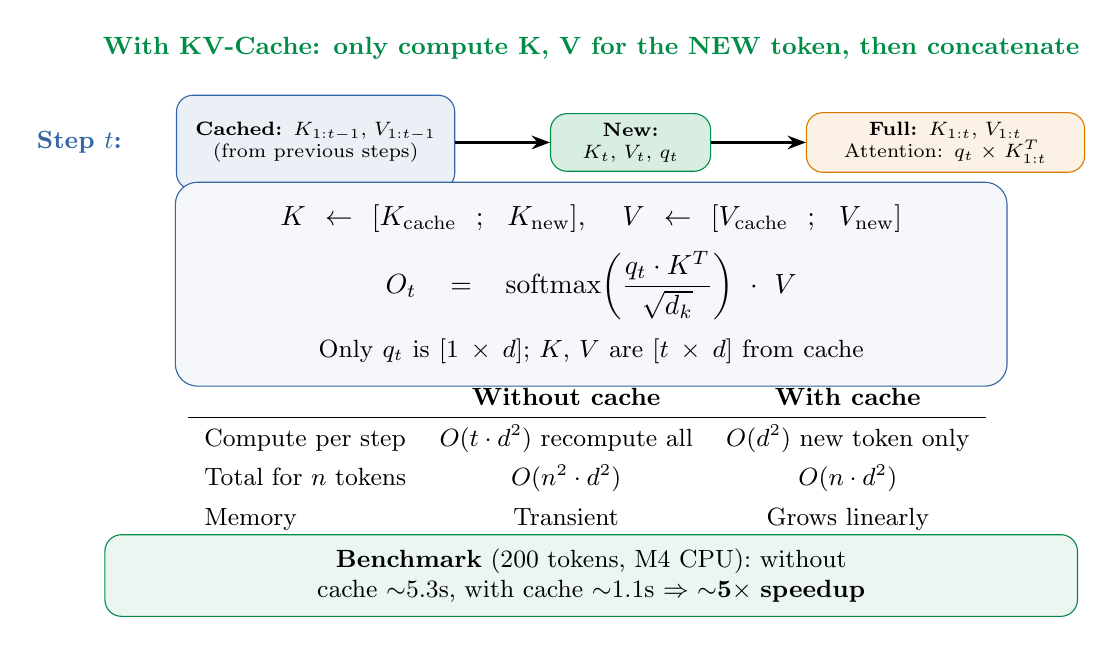
\begin{tikzpicture}
  \node[font=\small\bfseries, text=paramgreen] at (0, 3.5) {With KV-Cache: only compute K, V for the NEW token, then concatenate};

  % With cache diagram
  \node[font=\small\bfseries, text=popblue] at (-6.5, 2.3) {Step $t$:};

  % Cached K, V
  \node[draw=popblue, fill=popblue!10, rounded corners=6pt, minimum width=3.5cm, minimum height=1.2cm, text width=3.3cm, align=center, font=\scriptsize] (cache) at (-3.5, 2.3) {
    \textbf{Cached:} $K_{1:t-1}$, $V_{1:t-1}$\\(from previous steps)
  };

  % New token
  \node[draw=paramgreen, fill=paramgreen!15, rounded corners=6pt, minimum width=2cm, font=\scriptsize, text width=1.8cm, align=center] (new) at (0.5, 2.3) {
    \textbf{New:}\\$K_t$, $V_t$, $q_t$
  };

  % Concatenate
  \node[draw=orange1, fill=orange1!10, rounded corners=6pt, minimum width=3.5cm, font=\scriptsize, text width=3.3cm, align=center] (concat) at (4.5, 2.3) {
    \textbf{Full:} $K_{1:t}$, $V_{1:t}$\\Attention: $q_t \times K_{1:t}^T$
  };

  \draw[-Stealth, thick] (cache) -- (new);
  \draw[-Stealth, thick] (new) -- (concat);

  % Formula
  \node[draw=popblue, fill=popblue!5, rounded corners=8pt, inner sep=8pt, text width=10cm, align=center] at (0, 0.5) {
    {\normalsize $K \leftarrow [K_{\text{cache}} \;;\; K_{\text{new}}]$, \quad $V \leftarrow [V_{\text{cache}} \;;\; V_{\text{new}}]$}\\[6pt]
    {\normalsize $O_t = \text{softmax}\!\left(\dfrac{q_t \cdot K^T}{\sqrt{d_k}}\right) \cdot V$}\\[6pt]
    {\small Only $q_t$ is $[1 \times d]$; $K$, $V$ are $[t \times d]$ from cache}
  };

  % Complexity comparison
  \renewcommand{\arraystretch}{1.3}
  \node at (0, -1.7) {
    {\small
    \begin{tabular}{l c c}
      & \textbf{Without cache} & \textbf{With cache} \\
      \hline
      Compute per step & $O(t \cdot d^2)$ recompute all & $O(d^2)$ new token only \\
      Total for $n$ tokens & $O(n^2 \cdot d^2)$ & $O(n \cdot d^2)$ \\
      Memory & Transient & Grows linearly \\
    \end{tabular}
    }
  };

  % Speed numbers
  \node[draw=paramgreen, fill=paramgreen!8, rounded corners=6pt, text width=12cm, align=center, inner sep=5pt, font=\small] at (0, -3.2) {
    \textbf{Benchmark} (200 tokens, M4 CPU): without cache $\sim$5.3s, with cache $\sim$1.1s $\Rightarrow$ \textbf{$\sim$5$\times$ speedup}
  };
\end{tikzpicture}
\end{center}
\end{frame}

% ============================================================
% PREFILL vs DECODE
% ============================================================
\begin{frame}
\frametitle{Two phases of inference: prefill vs.\ decode}

\begin{center}
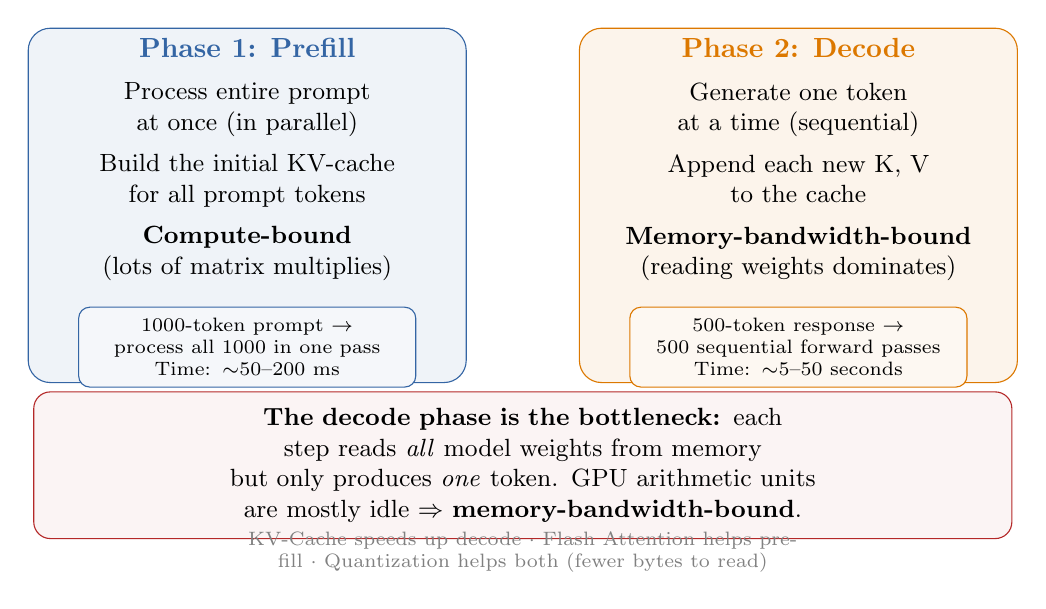
\begin{tikzpicture}
  % Prefill
  \node[draw=popblue, fill=popblue!8, rounded corners=8pt, minimum width=5.5cm, minimum height=4.5cm, text width=5cm, align=center, inner sep=8pt] at (-3.5, 1) {};
  \node[font=\normalsize\bfseries, text=popblue] at (-3.5, 3) {Phase 1: Prefill};

  \node[font=\small, text width=4.5cm, align=center] at (-3.5, 1.3) {
    Process entire prompt\\at once (in parallel)\\[4pt]
    Build the initial KV-cache\\for all prompt tokens\\[4pt]
    \textbf{Compute-bound}\\(lots of matrix multiplies)
  };
  \node[draw=popblue, fill=popblue!5, rounded corners=4pt, font=\scriptsize, text width=4cm, align=center, inner sep=4pt] at (-3.5, -0.8) {
    1000-token prompt $\to$\\process all 1000 in one pass\\Time: $\sim$50--200 ms
  };

  % Decode
  \node[draw=orange1, fill=orange1!8, rounded corners=8pt, minimum width=5.5cm, minimum height=4.5cm, text width=5cm, align=center, inner sep=8pt] at (3.5, 1) {};
  \node[font=\normalsize\bfseries, text=orange1] at (3.5, 3) {Phase 2: Decode};

  \node[font=\small, text width=4.5cm, align=center] at (3.5, 1.3) {
    Generate one token\\at a time (sequential)\\[4pt]
    Append each new K, V\\to the cache\\[4pt]
    \textbf{Memory-bandwidth-bound}\\(reading weights dominates)
  };
  \node[draw=orange1, fill=orange1!5, rounded corners=4pt, font=\scriptsize, text width=4cm, align=center, inner sep=4pt] at (3.5, -0.8) {
    500-token response $\to$\\500 sequential forward passes\\Time: $\sim$5--50 seconds
  };

  % Key insight
  \node[draw=warnred, fill=warnred!5, rounded corners=6pt, text width=12cm, align=center, inner sep=6pt, font=\small] at (0, -2.3) {
    \textbf{The decode phase is the bottleneck:} each step reads \emph{all} model weights from memory\\
    but only produces \emph{one} token. GPU arithmetic units are mostly idle $\Rightarrow$ \textbf{memory-bandwidth-bound}.
  };

  % Optimization targets
  \node[font=\scriptsize, text=gray, text width=12cm, align=center] at (0, -3.4) {
    KV-Cache speeds up decode $\cdot$ Flash Attention helps prefill $\cdot$ Quantization helps both (fewer bytes to read)
  };
\end{tikzpicture}
\end{center}
\end{frame}

% ============================================================
% KV-CACHE MEMORY COST
% ============================================================
\begin{frame}
\frametitle{KV-Cache memory cost}

\begin{center}
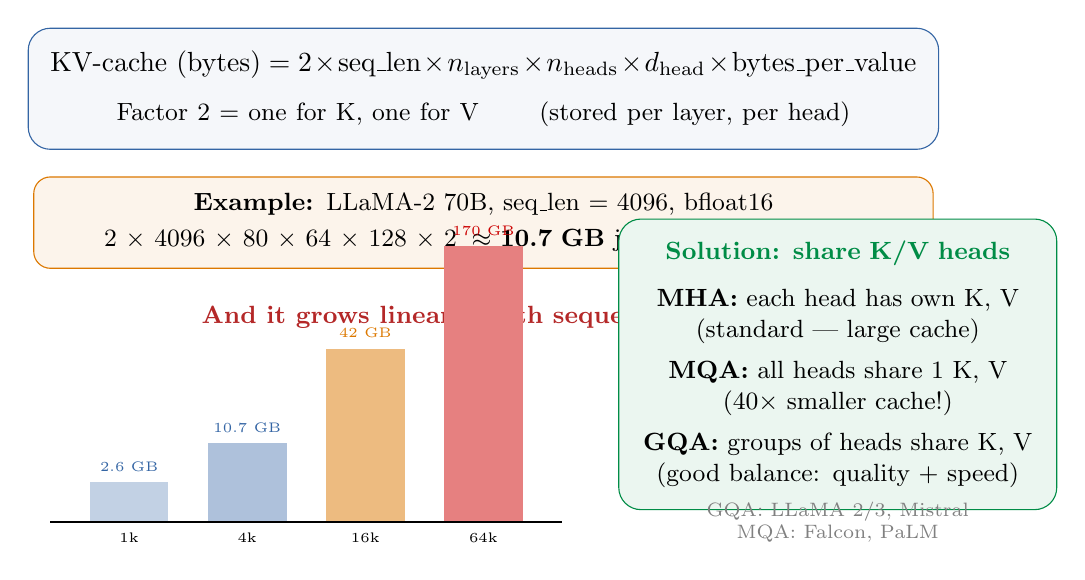
\begin{tikzpicture}
  % Formula
  \node[draw=popblue, fill=popblue!5, rounded corners=8pt, inner sep=8pt, text width=11cm, align=center] at (0, 3) {
    {\normalsize $\text{KV-cache (bytes)} = 2 \times \text{seq\_len} \times n_{\text{layers}} \times n_{\text{heads}} \times d_{\text{head}} \times \text{bytes\_per\_value}$}\\[6pt]
    {\small Factor 2 = one for K, one for V \qquad (stored per layer, per head)}
  };

  % Example calculation
  \node[draw=orange1, fill=orange1!8, rounded corners=6pt, text width=11cm, align=center, inner sep=6pt, font=\small] at (0, 1.3) {
    \textbf{Example:} LLaMA-2 70B, seq\_len = 4096, bfloat16\\[2pt]
    $2 \times 4096 \times 80 \times 64 \times 128 \times 2 \approx$ \textbf{10.7 GB} just for the KV-cache!
  };

  % The problem grows
  \node[font=\small\bfseries, text=warnred] at (0, 0.1) {And it grows linearly with sequence length:};

  % Bars for different seq lengths
  \fill[popblue!30] (-5, -2.5) rectangle (-4, -2);
  \node[font=\tiny] at (-4.5, -2.7) {1k};
  \node[font=\tiny, text=popblue] at (-4.5, -1.8) {2.6 GB};

  \fill[popblue!40] (-3.5, -2.5) rectangle (-2.5, -1.5);
  \node[font=\tiny] at (-3, -2.7) {4k};
  \node[font=\tiny, text=popblue] at (-3, -1.3) {10.7 GB};

  \fill[orange1!50] (-2, -2.5) rectangle (-1, -0.3);
  \node[font=\tiny] at (-1.5, -2.7) {16k};
  \node[font=\tiny, text=orange1] at (-1.5, -0.1) {42 GB};

  \fill[sampred!50] (-0.5, -2.5) rectangle (0.5, 1);
  \node[font=\tiny] at (0, -2.7) {64k};
  \node[font=\tiny, text=sampred] at (0, 1.2) {170 GB};

  \draw[thick] (-5.5, -2.5) -- (1, -2.5);

  % Solution: MQA/GQA
  \node[draw=paramgreen, fill=paramgreen!8, rounded corners=8pt, text width=5cm, align=center, inner sep=8pt, font=\small] at (4.5, -0.5) {
    \textbf{\textcolor{paramgreen}{Solution: share K/V heads}}\\[6pt]
    \textbf{MHA:} each head has own K, V\\(standard --- large cache)\\[4pt]
    \textbf{MQA:} all heads share 1 K, V\\(40$\times$ smaller cache!)\\[4pt]
    \textbf{GQA:} groups of heads share K, V\\(good balance: quality + speed)
  };

  % Who uses what
  \node[font=\scriptsize, text=gray, text width=5cm, align=center] at (4.5, -2.5) {
    GQA: LLaMA 2/3, Mistral\\MQA: Falcon, PaLM
  };
\end{tikzpicture}
\end{center}
\end{frame}

% ============================================================
% MQA / GQA DEEP DIVE
% ============================================================
\begin{frame}
\frametitle{MHA vs.\ MQA vs.\ GQA}

\begin{center}
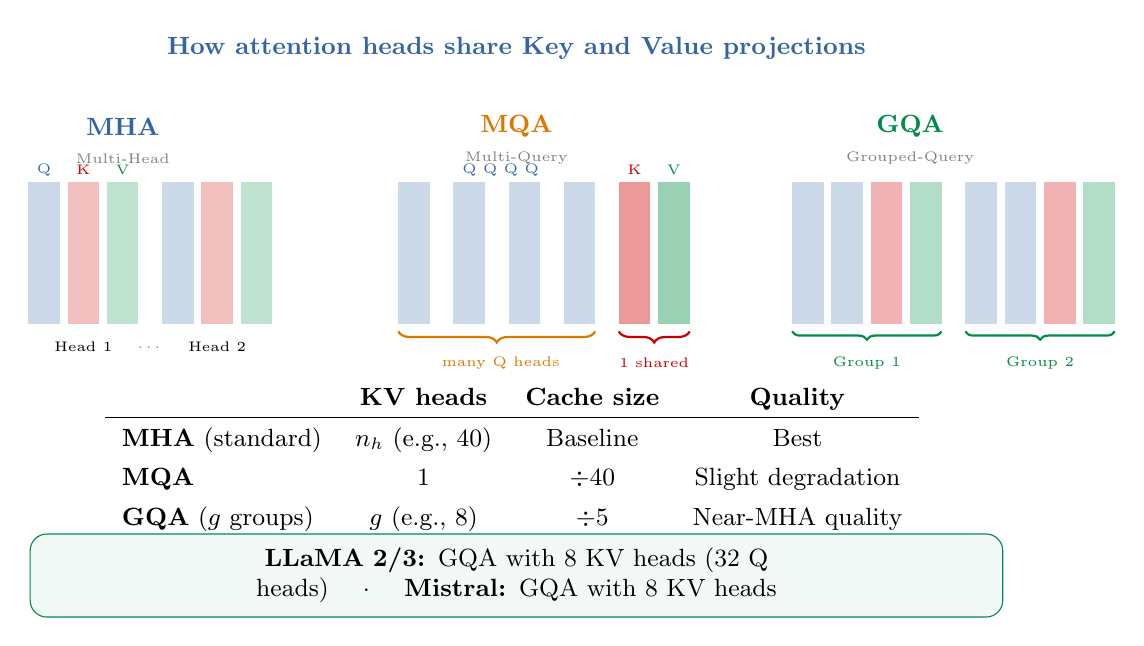
\begin{tikzpicture}
  \node[font=\small\bfseries, text=popblue] at (0, 3.5) {How attention heads share Key and Value projections};

  % MHA
  \node[font=\small\bfseries, text=popblue] at (-5, 2.5) {MHA};
  \node[font=\tiny, text=gray] at (-5, 2.1) {Multi-Head};

  % MHA heads - each with own Q, K, V
  \fill[popblue!25] (-6.2, 0) rectangle (-5.8, 1.8);
  \fill[sampred!25] (-5.7, 0) rectangle (-5.3, 1.8);
  \fill[paramgreen!25] (-5.2, 0) rectangle (-4.8, 1.8);

  \fill[popblue!25] (-4.5, 0) rectangle (-4.1, 1.8);
  \fill[sampred!25] (-4.0, 0) rectangle (-3.6, 1.8);
  \fill[paramgreen!25] (-3.5, 0) rectangle (-3.1, 1.8);

  \node[font=\tiny] at (-5.5, -0.3) {Head 1};
  \node[font=\tiny] at (-3.8, -0.3) {Head 2};
  \node[font=\tiny, text=gray] at (-4.65, -0.3) {\ldots};
  \node[font=\tiny, text=popblue] at (-6.0, 1.95) {Q};
  \node[font=\tiny, text=sampred] at (-5.5, 1.95) {K};
  \node[font=\tiny, text=paramgreen] at (-5.0, 1.95) {V};

  % MQA
  \node[font=\small\bfseries, text=orange1] at (0, 2.5) {MQA};
  \node[font=\tiny, text=gray] at (0, 2.1) {Multi-Query};

  \fill[popblue!25] (-1.5, 0) rectangle (-1.1, 1.8);
  \fill[popblue!25] (-0.8, 0) rectangle (-0.4, 1.8);
  \fill[popblue!25] (-0.1, 0) rectangle (0.3, 1.8);
  \fill[popblue!25] (0.6, 0) rectangle (1.0, 1.8);

  % Shared K, V
  \fill[sampred!40] (1.3, 0) rectangle (1.7, 1.8);
  \fill[paramgreen!40] (1.8, 0) rectangle (2.2, 1.8);

  \node[font=\tiny, text=popblue] at (-0.2, 1.95) {Q Q Q Q};
  \node[font=\tiny, text=sampred] at (1.5, 1.95) {K};
  \node[font=\tiny, text=paramgreen] at (2.0, 1.95) {V};

  \draw[decorate, decoration={brace, amplitude=4pt, mirror}, thick, orange1] (-1.5, -0.1) -- (1.0, -0.1);
  \node[font=\tiny, text=orange1] at (-0.2, -0.5) {many Q heads};
  \draw[decorate, decoration={brace, amplitude=4pt, mirror}, thick, sampred] (1.3, -0.1) -- (2.2, -0.1);
  \node[font=\tiny, text=sampred] at (1.75, -0.5) {1 shared};

  % GQA
  \node[font=\small\bfseries, text=paramgreen] at (5, 2.5) {GQA};
  \node[font=\tiny, text=gray] at (5, 2.1) {Grouped-Query};

  % Group 1
  \fill[popblue!25] (3.5, 0) rectangle (3.9, 1.8);
  \fill[popblue!25] (4.0, 0) rectangle (4.4, 1.8);
  \fill[sampred!30] (4.5, 0) rectangle (4.9, 1.8);
  \fill[paramgreen!30] (5.0, 0) rectangle (5.4, 1.8);

  % Group 2
  \fill[popblue!25] (5.7, 0) rectangle (6.1, 1.8);
  \fill[popblue!25] (6.2, 0) rectangle (6.6, 1.8);
  \fill[sampred!30] (6.7, 0) rectangle (7.1, 1.8);
  \fill[paramgreen!30] (7.2, 0) rectangle (7.6, 1.8);

  \draw[decorate, decoration={brace, amplitude=3pt, mirror}, thick, paramgreen] (3.5, -0.1) -- (5.4, -0.1);
  \node[font=\tiny, text=paramgreen] at (4.45, -0.5) {Group 1};
  \draw[decorate, decoration={brace, amplitude=3pt, mirror}, thick, paramgreen] (5.7, -0.1) -- (7.6, -0.1);
  \node[font=\tiny, text=paramgreen] at (6.65, -0.5) {Group 2};

  % Comparison table
  \renewcommand{\arraystretch}{1.3}
  \node at (0, -1.7) {
    {\small
    \begin{tabular}{l c c c}
      & \textbf{KV heads} & \textbf{Cache size} & \textbf{Quality} \\
      \hline
      \textbf{MHA} (standard) & $n_h$ (e.g., 40) & Baseline & Best \\
      \textbf{MQA} & 1 & $\div 40$ & Slight degradation \\
      \textbf{GQA} ($g$ groups) & $g$ (e.g., 8) & $\div 5$ & Near-MHA quality \\
    \end{tabular}
    }
  };

  % Models
  \node[draw=paramgreen, fill=paramgreen!5, rounded corners=6pt, text width=12cm, align=center, inner sep=5pt, font=\small] at (0, -3.2) {
    \textbf{LLaMA 2/3:} GQA with 8 KV heads (32 Q heads) \quad $\cdot$ \quad \textbf{Mistral:} GQA with 8 KV heads
  };
\end{tikzpicture}
\end{center}
\end{frame}

% ============================================================
% FLASH ATTENTION
% ============================================================
\begin{frame}
\frametitle{Flash Attention}

\begin{center}
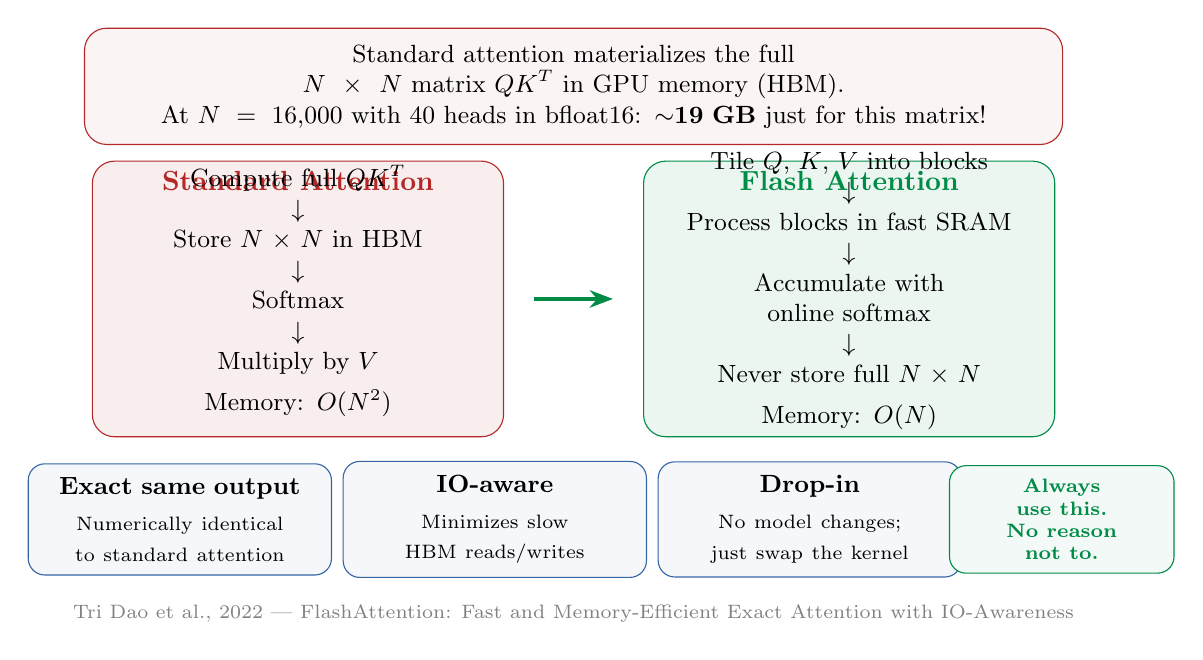
\begin{tikzpicture}
  % The problem
  \node[draw=warnred, fill=warnred!5, rounded corners=8pt, text width=12cm, align=center, inner sep=6pt, font=\small] at (0, 3.2) {
    Standard attention materializes the full $N \times N$ matrix $QK^T$ in GPU memory (HBM).\\
    At $N = 16{,}000$ with 40 heads in bfloat16: $\sim$\textbf{19 GB} just for this matrix!
  };

  % Standard vs Flash
  \node[draw=warnred, fill=warnred!8, rounded corners=8pt, minimum width=5.2cm, minimum height=3.5cm, text width=4.8cm, align=center, inner sep=6pt] at (-3.5, 0.5) {};
  \node[font=\normalsize\bfseries, text=warnred] at (-3.5, 2) {Standard Attention};
  \node[font=\small, text width=4.5cm, align=center] at (-3.5, 0.6) {
    Compute full $QK^T$\\$\downarrow$\\Store $N \times N$ in HBM\\$\downarrow$\\Softmax\\$\downarrow$\\Multiply by $V$\\[4pt]
    Memory: $O(N^2)$
  };

  \node[draw=paramgreen, fill=paramgreen!8, rounded corners=8pt, minimum width=5.2cm, minimum height=3.5cm, text width=4.8cm, align=center, inner sep=6pt] at (3.5, 0.5) {};
  \node[font=\normalsize\bfseries, text=paramgreen] at (3.5, 2) {Flash Attention};
  \node[font=\small, text width=4.5cm, align=center] at (3.5, 0.6) {
    Tile $Q$, $K$, $V$ into blocks\\$\downarrow$\\Process blocks in fast SRAM\\$\downarrow$\\Accumulate with online softmax\\$\downarrow$\\Never store full $N \times N$\\[4pt]
    Memory: $O(N)$
  };

  \draw[-Stealth, very thick, paramgreen] (-0.5, 0.5) -- (0.5, 0.5);

  % Key properties
  \node[draw=popblue, fill=popblue!5, rounded corners=6pt, text width=3.5cm, align=center, inner sep=5pt, font=\small] at (-5, -2.3) {
    \textbf{Exact same output}\\[2pt]
    {\scriptsize Numerically identical to standard attention}
  };
  \node[draw=popblue, fill=popblue!5, rounded corners=6pt, text width=3.5cm, align=center, inner sep=5pt, font=\small] at (-1, -2.3) {
    \textbf{IO-aware}\\[2pt]
    {\scriptsize Minimizes slow HBM reads/writes}
  };
  \node[draw=popblue, fill=popblue!5, rounded corners=6pt, text width=3.5cm, align=center, inner sep=5pt, font=\small] at (3, -2.3) {
    \textbf{Drop-in}\\[2pt]
    {\scriptsize No model changes; just swap the kernel}
  };

  % Recommendation
  \node[draw=paramgreen, fill=paramgreen!5, rounded corners=6pt, text width=2.5cm, align=center, inner sep=5pt, font=\scriptsize\bfseries, text=paramgreen] at (6.2, -2.3) {
    Always\\use this.\\No reason\\not to.
  };

  % Citation
  \node[font=\scriptsize, text=gray] at (0, -3.5) {Tri Dao et al., 2022 --- FlashAttention: Fast and Memory-Efficient Exact Attention with IO-Awareness};
\end{tikzpicture}
\end{center}
\end{frame}

% ============================================================
% GPU MEMORY HIERARCHY
% ============================================================
\begin{frame}
\frametitle{Why Flash Attention works: the GPU memory hierarchy}

\begin{center}
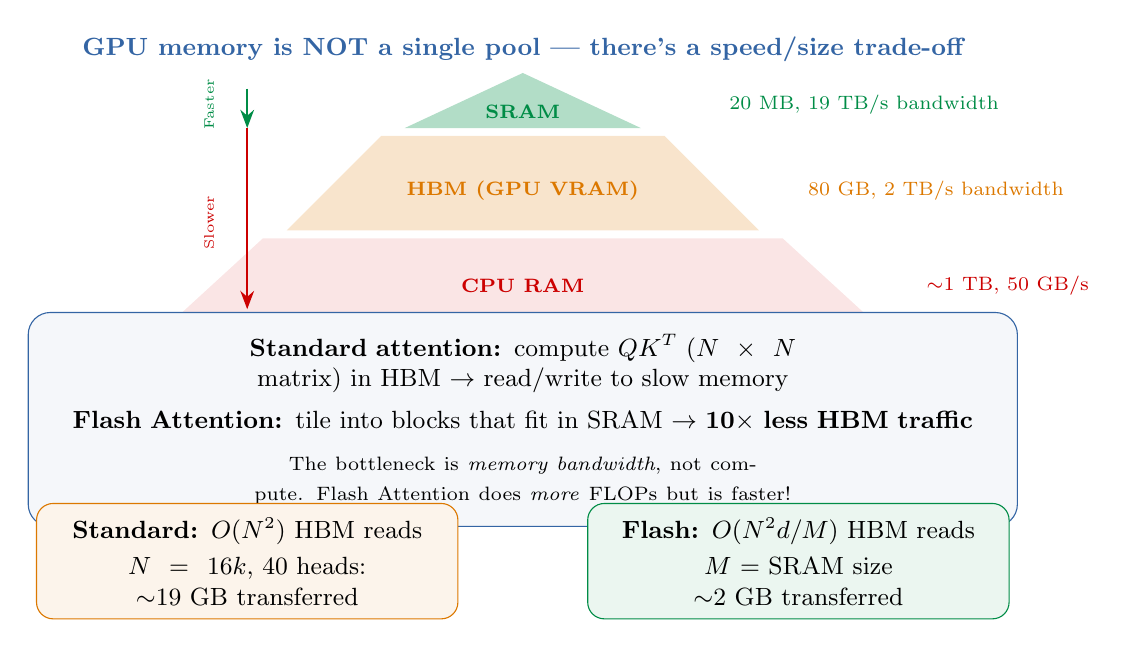
\begin{tikzpicture}
  % Memory hierarchy pyramid
  \node[font=\small\bfseries, text=popblue] at (0, 3.5) {GPU memory is NOT a single pool --- there's a speed/size trade-off};

  % SRAM (fast, small)
  \fill[paramgreen!30] (-1.5, 2.5) -- (1.5, 2.5) -- (0, 3.2) -- cycle;
  \node[font=\scriptsize\bfseries, text=paramgreen] at (0, 2.7) {SRAM};

  % HBM (slower, bigger)
  \fill[orange1!20] (-3, 1.2) -- (3, 1.2) -- (1.8, 2.4) -- (-1.8, 2.4) -- cycle;
  \node[font=\scriptsize\bfseries, text=orange1] at (0, 1.7) {HBM (GPU VRAM)};

  % CPU RAM (slowest, biggest)
  \fill[sampred!10] (-4.5, 0) -- (4.5, 0) -- (3.3, 1.1) -- (-3.3, 1.1) -- cycle;
  \node[font=\scriptsize\bfseries, text=sampred] at (0, 0.5) {CPU RAM};

  % Annotations - right side
  \node[font=\scriptsize, text=paramgreen, anchor=west] at (2.5, 2.8) {20 MB, 19 TB/s bandwidth};
  \node[font=\scriptsize, text=orange1, anchor=west] at (3.5, 1.7) {80 GB, 2 TB/s bandwidth};
  \node[font=\scriptsize, text=sampred, anchor=west] at (5, 0.5) {$\sim$1 TB, 50 GB/s};

  % Speed arrows
  \draw[-Stealth, thick, paramgreen] (-3.5, 3) -- (-3.5, 2.5);
  \node[font=\tiny, text=paramgreen, rotate=90, anchor=south] at (-3.8, 2.8) {Faster};
  \draw[-Stealth, thick, sampred] (-3.5, 2.5) -- (-3.5, 0.2);
  \node[font=\tiny, text=sampred, rotate=90, anchor=south] at (-3.8, 1.3) {Slower};

  % The insight
  \node[draw=popblue, fill=popblue!5, rounded corners=8pt, text width=12cm, align=center, inner sep=8pt, font=\small] at (0, -1.2) {
    \textbf{Standard attention:} compute $QK^T$ ($N \times N$ matrix) in HBM $\to$ read/write to slow memory\\[4pt]
    \textbf{Flash Attention:} tile into blocks that fit in SRAM $\to$ \textbf{10$\times$ less HBM traffic}\\[4pt]
    {\scriptsize The bottleneck is \emph{memory bandwidth}, not compute. Flash Attention does \emph{more} FLOPs but is faster!}
  };

  % Numbers
  \node[draw=orange1, fill=orange1!8, rounded corners=6pt, text width=5cm, align=center, inner sep=5pt, font=\small] at (-3.5, -3) {
    \textbf{Standard:} $O(N^2)$ HBM reads\\[2pt]
    $N = 16k$, 40 heads:\\$\sim$19 GB transferred
  };
  \node[draw=paramgreen, fill=paramgreen!8, rounded corners=6pt, text width=5cm, align=center, inner sep=5pt, font=\small] at (3.5, -3) {
    \textbf{Flash:} $O(N^2 d / M)$ HBM reads\\[2pt]
    $M$ = SRAM size\\$\sim$2 GB transferred
  };
\end{tikzpicture}
\end{center}
\end{frame}

% ============================================================
% PART II HEADER
% ============================================================
\begin{frame}
\begin{center}
\vspace{1.5cm}
{\Huge \textcolor{orange1}{Part II}}

\vspace{0.5cm}
{\Large Quantization}

\vspace{0.5cm}
{\normalsize Reducing precision to reduce memory}
\end{center}
\end{frame}

% ============================================================
% WHAT IS QUANTIZATION
% ============================================================
\begin{frame}
\frametitle{What is quantization?}

\begin{center}
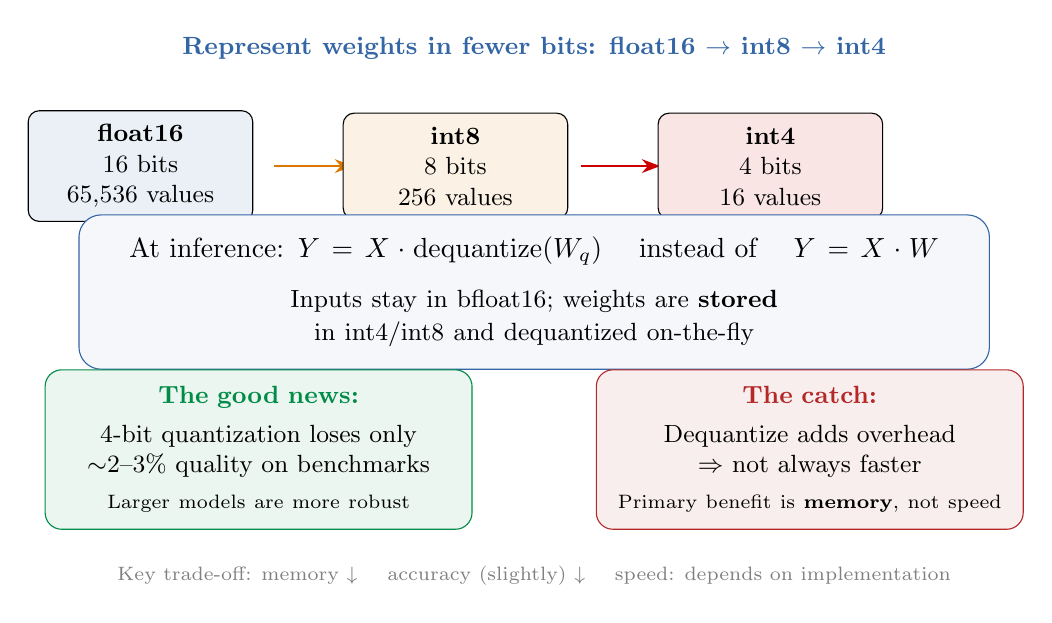
\begin{tikzpicture}
  % Idea
  \node[font=\small\bfseries, text=popblue] at (0, 3.5) {Represent weights in fewer bits: float16 $\to$ int8 $\to$ int4};

  % Precision visualization
  \node[draw, rounded corners=4pt, fill=popblue!10, text width=2.5cm, align=center, inner sep=5pt, font=\small] at (-5, 2) {
    \textbf{float16}\\16 bits\\65,536 values
  };
  \draw[-Stealth, thick, orange1] (-3.3, 2) -- (-2.3, 2);
  \node[draw, rounded corners=4pt, fill=orange1!10, text width=2.5cm, align=center, inner sep=5pt, font=\small] at (-1, 2) {
    \textbf{int8}\\8 bits\\256 values
  };
  \draw[-Stealth, thick, sampred] (0.6, 2) -- (1.6, 2);
  \node[draw, rounded corners=4pt, fill=sampred!10, text width=2.5cm, align=center, inner sep=5pt, font=\small] at (3, 2) {
    \textbf{int4}\\4 bits\\16 values
  };

  % At inference
  \node[draw=popblue, fill=popblue!5, rounded corners=8pt, inner sep=8pt, text width=11cm, align=center] at (0, 0.4) {
    At inference: $Y = X \cdot \text{dequantize}(W_q)$ \quad instead of \quad $Y = X \cdot W$\\[6pt]
    {\small Inputs stay in bfloat16; weights are \textbf{stored} in int4/int8 and dequantized on-the-fly}
  };

  % Quality vs compression
  \node[draw=paramgreen, fill=paramgreen!8, rounded corners=6pt, text width=5cm, align=center, inner sep=6pt, font=\small] at (-3.5, -1.6) {
    \textbf{\textcolor{paramgreen}{The good news:}}\\[3pt]
    4-bit quantization loses only\\$\sim$2--3\% quality on benchmarks\\[2pt]
    {\scriptsize Larger models are more robust}
  };

  \node[draw=warnred, fill=warnred!8, rounded corners=6pt, text width=5cm, align=center, inner sep=6pt, font=\small] at (3.5, -1.6) {
    \textbf{\textcolor{warnred}{The catch:}}\\[3pt]
    Dequantize adds overhead\\$\Rightarrow$ not always faster\\[2pt]
    {\scriptsize Primary benefit is \textbf{memory}, not speed}
  };

  % Bottom note
  \node[font=\scriptsize, text=gray] at (0, -3.2) {
    Key trade-off: memory $\downarrow$ \quad accuracy (slightly) $\downarrow$ \quad speed: depends on implementation
  };
\end{tikzpicture}
\end{center}
\end{frame}

% ============================================================
% QUANTIZATION MATH
% ============================================================
\begin{frame}
\frametitle{The math of quantization}

\begin{center}
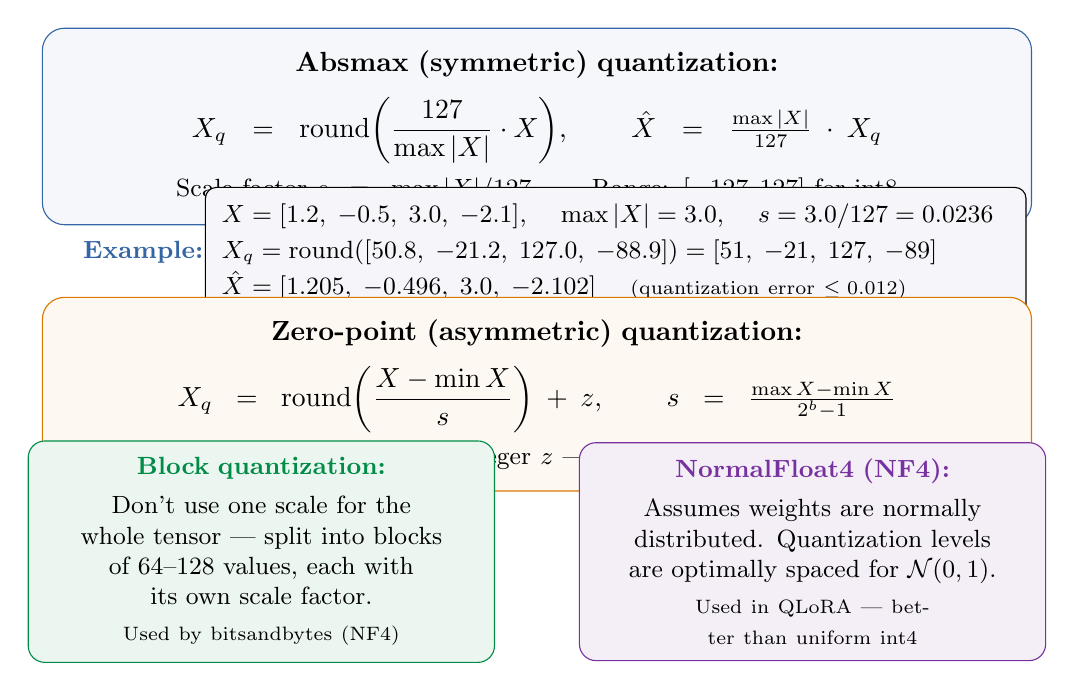
\begin{tikzpicture}
  % Absmax quantization
  \node[draw=popblue, fill=popblue!5, rounded corners=8pt, inner sep=8pt, text width=12cm, align=center] at (0, 3.1) {
    \textbf{Absmax (symmetric) quantization:}\\[6pt]
    {\normalsize $\displaystyle X_q = \text{round}\!\left(\frac{127}{\max |X|} \cdot X\right)$, \qquad $\hat{X} = \frac{\max |X|}{127} \cdot X_q$}\\[4pt]
    {\small Scale factor $s = \max |X| / 127$ \qquad Range: $[-127, 127]$ for int8}
  };

  % Worked example
  \node[font=\small\bfseries, text=popblue] at (-5, 1.5) {Example:};
  \node[draw, rounded corners=4pt, fill=lightbg, text width=10cm, align=left, inner sep=6pt, font=\small] at (1, 1.5) {
    $X = [1.2, \;-0.5, \;3.0, \;-2.1]$, \quad $\max |X| = 3.0$, \quad $s = 3.0/127 = 0.0236$\\[2pt]
    $X_q = \text{round}([50.8,\; -21.2,\; 127.0,\; -88.9]) = [51,\; -21,\; 127,\; -89]$\\[2pt]
    $\hat{X} = [1.205,\; -0.496,\; 3.0,\; -2.102]$ \quad {\scriptsize (quantization error $\leq 0.012$)}
  };

  % Zero-point (asymmetric)
  \node[draw=orange1, fill=orange1!5, rounded corners=8pt, inner sep=8pt, text width=12cm, align=center] at (0, -0.3) {
    \textbf{Zero-point (asymmetric) quantization:}\\[6pt]
    {\normalsize $\displaystyle X_q = \text{round}\!\left(\frac{X - \min X}{s}\right) + z$, \qquad $s = \frac{\max X - \min X}{2^b - 1}$}\\[4pt]
    {\small Shifts the range so zero maps to integer $z$ --- better for asymmetric distributions}
  };

  % Block quantization
  \node[draw=paramgreen, fill=paramgreen!8, rounded corners=6pt, text width=5.5cm, align=center, inner sep=6pt, font=\small] at (-3.5, -2.3) {
    \textbf{\textcolor{paramgreen}{Block quantization:}}\\[3pt]
    Don't use one scale for the\\whole tensor --- split into blocks\\of 64--128 values, each with\\its own scale factor.\\[2pt]
    {\scriptsize Used by bitsandbytes (NF4)}
  };

  % NF4
  \node[draw=violet1, fill=violet1!8, rounded corners=6pt, text width=5.5cm, align=center, inner sep=6pt, font=\small] at (3.5, -2.3) {
    \textbf{\textcolor{violet1}{NormalFloat4 (NF4):}}\\[3pt]
    Assumes weights are normally\\distributed. Quantization levels\\are optimally spaced for $\mathcal{N}(0, 1)$.\\[2pt]
    {\scriptsize Used in QLoRA --- better than uniform int4}
  };
\end{tikzpicture}
\end{center}
\end{frame}

% ============================================================
% PTQ vs QAT
% ============================================================
\begin{frame}
\frametitle{When to quantize: PTQ vs.\ QAT}

\begin{center}
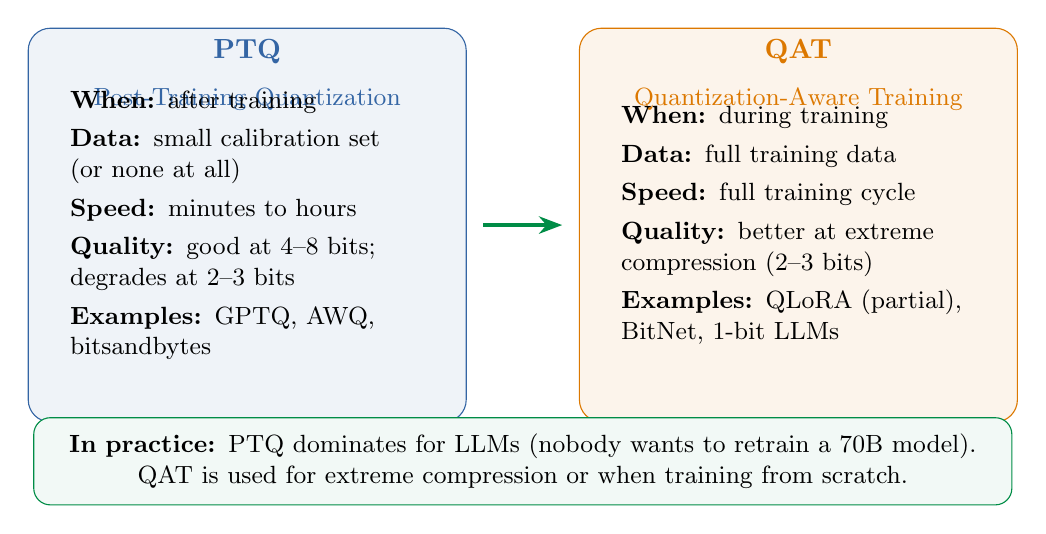
\begin{tikzpicture}
  % PTQ
  \node[draw=popblue, fill=popblue!8, rounded corners=8pt, minimum width=5.5cm, minimum height=5cm, text width=5cm, align=center, inner sep=8pt] at (-3.5, 0.5) {};
  \node[font=\normalsize\bfseries, text=popblue] at (-3.5, 2.7) {PTQ};
  \node[font=\small, text=popblue] at (-3.5, 2.1) {Post-Training Quantization};

  \node[font=\small, text width=4.5cm, align=left] at (-3.5, 0.5) {
    \textbf{When:} after training\\[3pt]
    \textbf{Data:} small calibration set\\(or none at all)\\[3pt]
    \textbf{Speed:} minutes to hours\\[3pt]
    \textbf{Quality:} good at 4--8 bits;\\degrades at 2--3 bits\\[3pt]
    \textbf{Examples:} GPTQ, AWQ,\\bitsandbytes
  };

  % QAT
  \node[draw=orange1, fill=orange1!8, rounded corners=8pt, minimum width=5.5cm, minimum height=5cm, text width=5cm, align=center, inner sep=8pt] at (3.5, 0.5) {};
  \node[font=\normalsize\bfseries, text=orange1] at (3.5, 2.7) {QAT};
  \node[font=\small, text=orange1] at (3.5, 2.1) {Quantization-Aware Training};

  \node[font=\small, text width=4.5cm, align=left] at (3.5, 0.5) {
    \textbf{When:} during training\\[3pt]
    \textbf{Data:} full training data\\[3pt]
    \textbf{Speed:} full training cycle\\[3pt]
    \textbf{Quality:} better at extreme\\compression (2--3 bits)\\[3pt]
    \textbf{Examples:} QLoRA (partial),\\BitNet, 1-bit LLMs
  };

  % Arrow
  \draw[-Stealth, very thick, paramgreen] (-0.5, 0.5) -- (0.5, 0.5);

  % Bottom
  \node[draw=paramgreen, fill=paramgreen!5, rounded corners=6pt, text width=12cm, align=center, inner sep=6pt, font=\small] at (0, -2.5) {
    \textbf{In practice:} PTQ dominates for LLMs (nobody wants to retrain a 70B model).\\
    QAT is used for extreme compression or when training from scratch.
  };
\end{tikzpicture}
\end{center}
\end{frame}

% ============================================================
% QUANTIZATION METHODS
% ============================================================
\begin{frame}
\frametitle{Quantization methods compared}

\vspace{-0.2cm}
\renewcommand{\arraystretch}{1.4}
\begin{center}
{\small
\begin{tabular}{>{\bfseries}l c c c c}
  \textbf{Method} & \textbf{Calibration} & \textbf{Bits} & \textbf{Speed} & \textbf{Best for} \\
  \hline
  \textcolor{popblue}{bitsandbytes} & None & 4, 8 & Slower & Quick experiments, QLoRA \\[2pt]
  \textcolor{paramgreen}{GPTQ} & Required & 2--8 & 2$\times$ faster & Production deployment \\[2pt]
  \textcolor{orange1}{AWQ} & Required & 3--4 & Fast & Production, multi-modal \\
  \hline
\end{tabular}
}
\end{center}

\vspace{0.2cm}
\begin{center}
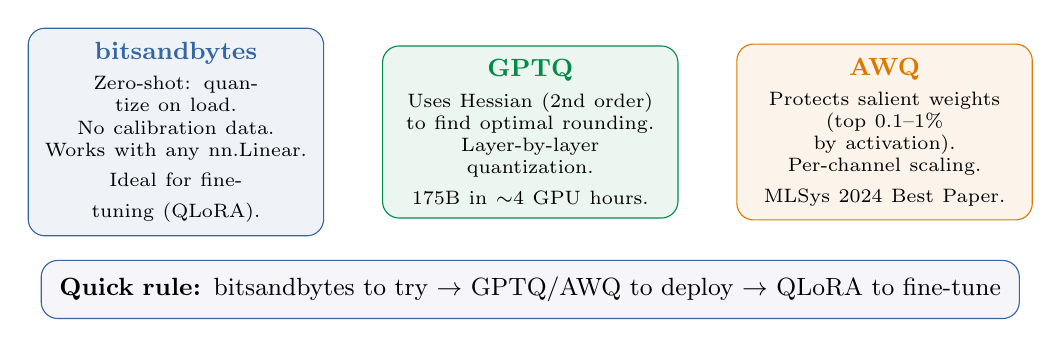
\begin{tikzpicture}
  % bitsandbytes
  \node[draw=popblue, fill=popblue!8, rounded corners=6pt, text width=3.4cm, align=center, inner sep=5pt, font=\small] at (-4.5, 0.5) {
    \textbf{\textcolor{popblue}{bitsandbytes}}\\[3pt]
    {\scriptsize Zero-shot: quantize on load.\\No calibration data.\\Works with any nn.Linear.\\Ideal for fine-tuning (QLoRA).}
  };

  % GPTQ
  \node[draw=paramgreen, fill=paramgreen!8, rounded corners=6pt, text width=3.4cm, align=center, inner sep=5pt, font=\small] at (0, 0.5) {
    \textbf{\textcolor{paramgreen}{GPTQ}}\\[3pt]
    {\scriptsize Uses Hessian (2nd order)\\to find optimal rounding.\\Layer-by-layer quantization.\\175B in $\sim$4 GPU hours.}
  };

  % AWQ
  \node[draw=orange1, fill=orange1!8, rounded corners=6pt, text width=3.4cm, align=center, inner sep=5pt, font=\small] at (4.5, 0.5) {
    \textbf{\textcolor{orange1}{AWQ}}\\[3pt]
    {\scriptsize Protects salient weights\\(top 0.1--1\% by activation).\\Per-channel scaling.\\MLSys 2024 Best Paper.}
  };

  % Bottom recommendation
  \node[draw=popblue, fill=lightbg, rounded corners=6pt, text width=12cm, align=center, inner sep=6pt, font=\small] at (0, -1.5) {
    \textbf{Quick rule:} bitsandbytes to try $\to$ GPTQ/AWQ to deploy $\to$ QLoRA to fine-tune
  };
\end{tikzpicture}
\end{center}
\end{frame}

% ============================================================
% GPTQ DEEP DIVE
% ============================================================
\begin{frame}
\frametitle{GPTQ --- optimal weight quantization}

\begin{center}
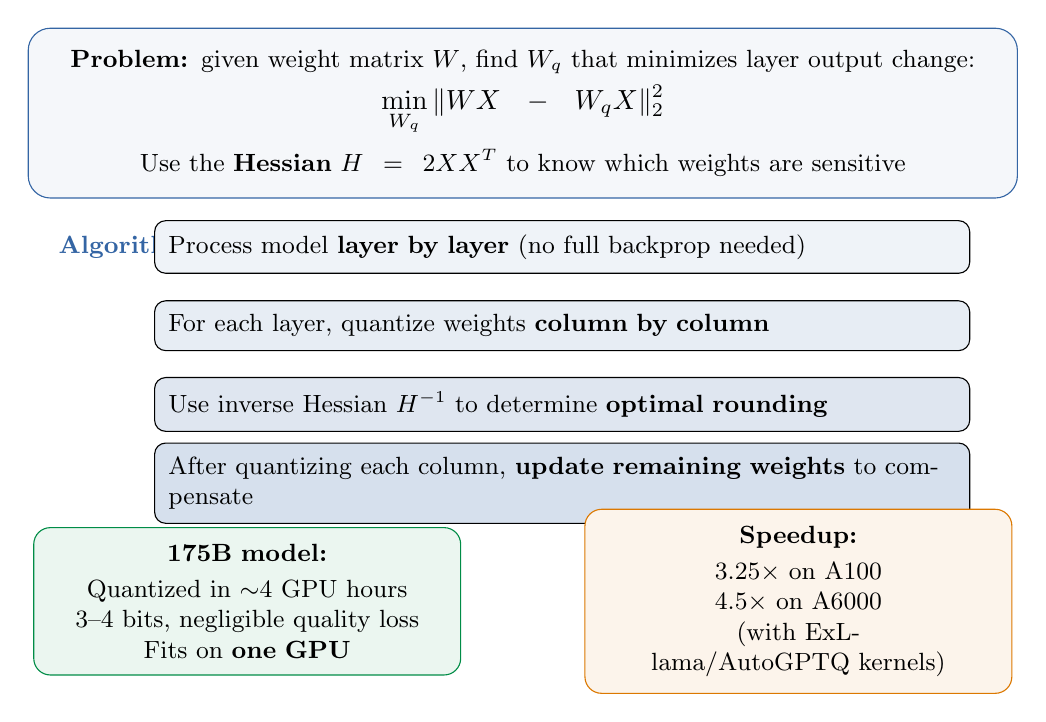
\begin{tikzpicture}
  % Core idea
  \node[draw=popblue, fill=popblue!5, rounded corners=8pt, text width=12cm, align=center, inner sep=8pt, font=\small] at (0, 3.2) {
    \textbf{Problem:} given weight matrix $W$, find $W_q$ that minimizes layer output change:\\[4pt]
    {\normalsize $\displaystyle \min_{W_q} \| WX - W_q X \|_2^2$}\\[4pt]
    {\small Use the \textbf{Hessian} $H = 2XX^T$ to know which weights are sensitive}
  };

  % Algorithm steps
  \node[font=\small\bfseries, text=popblue] at (-5, 1.5) {Algorithm:};

  \node[draw, rounded corners=4pt, fill=popblue!8, text width=10cm, align=left, inner sep=5pt, font=\small] at (0.5, 1.5) {
    Process model \textbf{layer by layer} (no full backprop needed)
  };
  \node[draw, rounded corners=4pt, fill=popblue!12, text width=10cm, align=left, inner sep=5pt, font=\small] at (0.5, 0.5) {
    For each layer, quantize weights \textbf{column by column}
  };
  \node[draw, rounded corners=4pt, fill=popblue!16, text width=10cm, align=left, inner sep=5pt, font=\small] at (0.5, -0.5) {
    Use inverse Hessian $H^{-1}$ to determine \textbf{optimal rounding}
  };
  \node[draw, rounded corners=4pt, fill=popblue!20, text width=10cm, align=left, inner sep=5pt, font=\small] at (0.5, -1.5) {
    After quantizing each column, \textbf{update remaining weights} to compensate
  };

  % Key results
  \node[draw=paramgreen, fill=paramgreen!8, rounded corners=6pt, text width=5cm, align=center, inner sep=6pt, font=\small] at (-3.5, -3) {
    \textbf{175B model:}\\[2pt]
    Quantized in $\sim$4 GPU hours\\3--4 bits, negligible quality loss\\Fits on \textbf{one GPU}
  };
  \node[draw=orange1, fill=orange1!8, rounded corners=6pt, text width=5cm, align=center, inner sep=6pt, font=\small] at (3.5, -3) {
    \textbf{Speedup:}\\[2pt]
    3.25$\times$ on A100\\4.5$\times$ on A6000\\(with ExLlama/AutoGPTQ kernels)
  };
\end{tikzpicture}
\end{center}
\end{frame}

% ============================================================
% QUANTIZATION BENCHMARKS
% ============================================================
\begin{frame}
\frametitle{Quantization benchmarks}

\vspace{-0.1cm}
\begin{center}
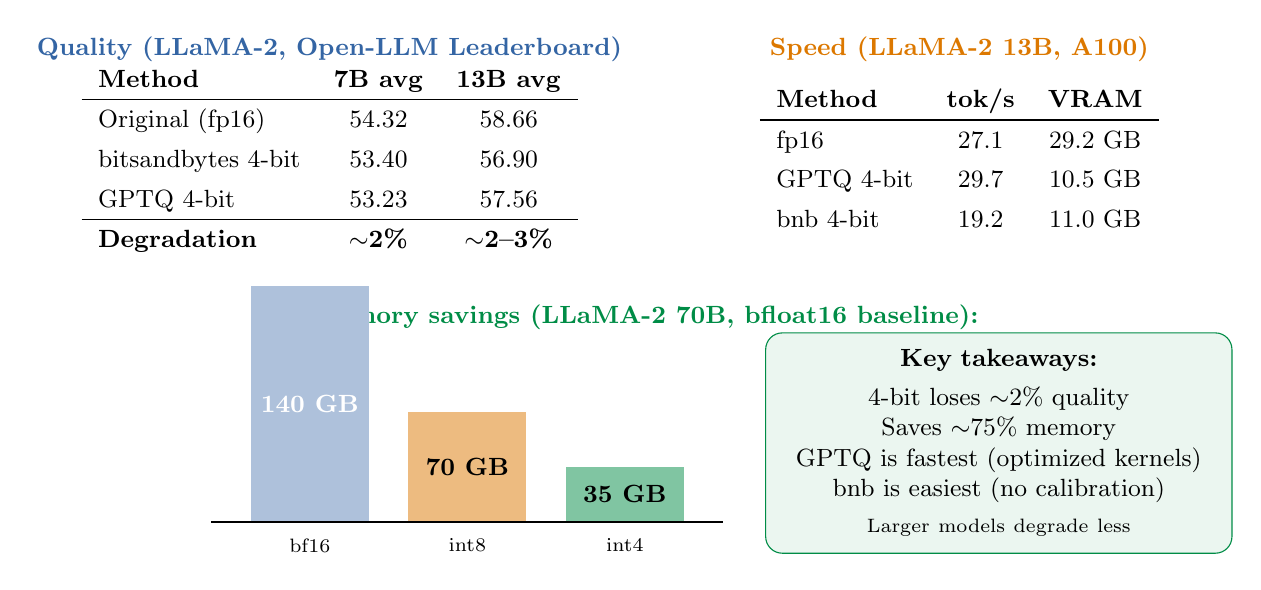
\begin{tikzpicture}
  % Quality benchmarks
  \node[font=\small\bfseries, text=popblue] at (-4, 3.5) {Quality (LLaMA-2, Open-LLM Leaderboard)};

  \node at (-4, 2.1) {
    {\small
    \renewcommand{\arraystretch}{1.3}
    \begin{tabular}{l c c}
      \textbf{Method} & \textbf{7B avg} & \textbf{13B avg} \\
      \hline
      Original (fp16) & 54.32 & 58.66 \\
      bitsandbytes 4-bit & 53.40 & 56.90 \\
      GPTQ 4-bit & 53.23 & 57.56 \\
      \hline
      \textbf{Degradation} & \textbf{$\sim$2\%} & \textbf{$\sim$2--3\%} \\
    \end{tabular}
    }
  };

  % Speed benchmarks
  \node[font=\small\bfseries, text=orange1] at (4, 3.5) {Speed (LLaMA-2 13B, A100)};

  \node at (4, 2.1) {
    {\small
    \renewcommand{\arraystretch}{1.3}
    \begin{tabular}{l c c}
      \textbf{Method} & \textbf{tok/s} & \textbf{VRAM} \\
      \hline
      fp16 & 27.1 & 29.2 GB \\
      GPTQ 4-bit & 29.7 & 10.5 GB \\
      bnb 4-bit & 19.2 & 11.0 GB \\
    \end{tabular}
    }
  };

  % Memory impact visual
  \node[font=\small\bfseries, text=paramgreen] at (0, 0.1) {Memory savings (LLaMA-2 70B, bfloat16 baseline):};

  % Bars
  \fill[popblue!40] (-5, -2.5) rectangle (-3.5, 0.5);
  \node[font=\small, text=white] at (-4.25, -1) {\textbf{140 GB}};
  \node[font=\scriptsize] at (-4.25, -2.8) {bf16};

  \fill[orange1!50] (-3, -2.5) rectangle (-1.5, -1.1);
  \node[font=\small] at (-2.25, -1.8) {\textbf{70 GB}};
  \node[font=\scriptsize] at (-2.25, -2.8) {int8};

  \fill[paramgreen!50] (-1, -2.5) rectangle (0.5, -1.8);
  \node[font=\small] at (-0.25, -2.15) {\textbf{35 GB}};
  \node[font=\scriptsize] at (-0.25, -2.8) {int4};

  \draw[thick] (-5.5, -2.5) -- (1, -2.5);

  % Takeaway
  \node[draw=paramgreen, fill=paramgreen!8, rounded corners=6pt, text width=5.5cm, align=center, inner sep=6pt, font=\small] at (4.5, -1.5) {
    \textbf{Key takeaways:}\\[3pt]
    4-bit loses $\sim$2\% quality\\Saves $\sim$75\% memory\\GPTQ is fastest (optimized kernels)\\bnb is easiest (no calibration)\\[2pt]
    {\scriptsize Larger models degrade less}
  };
\end{tikzpicture}
\end{center}
\end{frame}

% ============================================================
% AWQ DEEP DIVE
% ============================================================
\begin{frame}
\frametitle{AWQ --- protecting salient weights}

\begin{center}
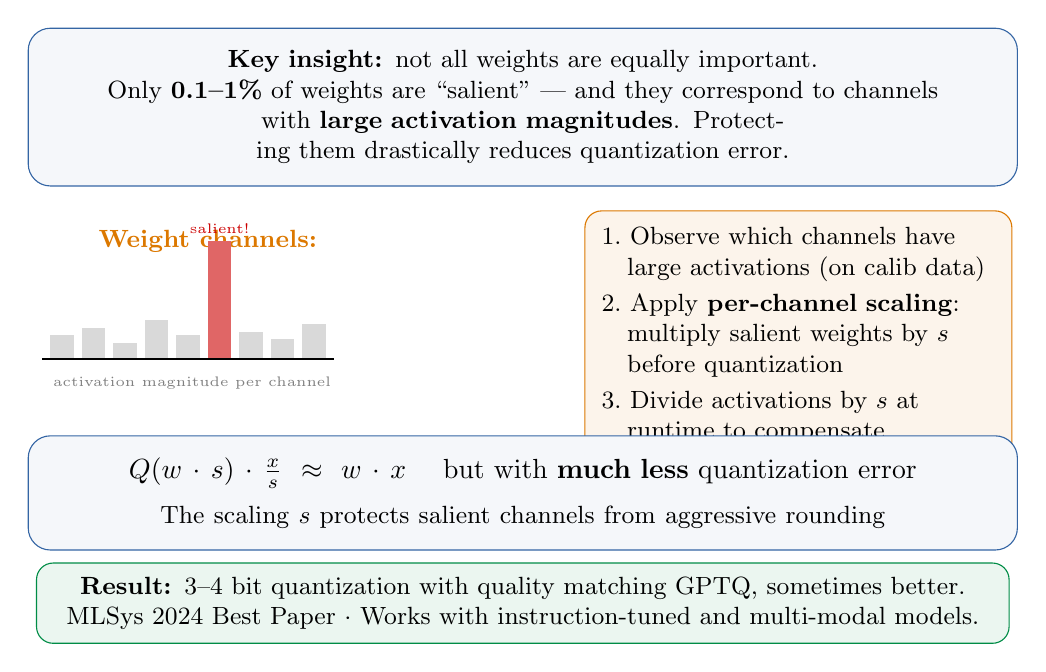
\begin{tikzpicture}
  % Key insight
  \node[draw=popblue, fill=popblue!5, rounded corners=8pt, text width=12cm, align=center, inner sep=8pt, font=\small] at (0, 3.2) {
    \textbf{Key insight:} not all weights are equally important.\\
    Only \textbf{0.1--1\%} of weights are ``salient'' --- and they correspond to channels\\
    with \textbf{large activation magnitudes}. Protecting them drastically reduces quantization error.
  };

  % Weight importance visualization
  \node[font=\small\bfseries, text=orange1] at (-4, 1.5) {Weight channels:};

  % Many unimportant weights (small bars)
  \fill[gray!30] (-6, 0) rectangle (-5.7, 0.3);
  \fill[gray!30] (-5.6, 0) rectangle (-5.3, 0.4);
  \fill[gray!30] (-5.2, 0) rectangle (-4.9, 0.2);
  \fill[gray!30] (-4.8, 0) rectangle (-4.5, 0.5);
  \fill[gray!30] (-4.4, 0) rectangle (-4.1, 0.3);
  % Salient weight (tall bar)
  \fill[sampred!60] (-4.0, 0) rectangle (-3.7, 1.5);
  \node[font=\tiny, text=sampred] at (-3.85, 1.65) {salient!};
  % More unimportant
  \fill[gray!30] (-3.6, 0) rectangle (-3.3, 0.35);
  \fill[gray!30] (-3.2, 0) rectangle (-2.9, 0.25);
  \fill[gray!30] (-2.8, 0) rectangle (-2.5, 0.45);

  \draw[thick] (-6.1, 0) -- (-2.4, 0);
  \node[font=\tiny, text=gray] at (-4.2, -0.3) {activation magnitude per channel};

  % The AWQ approach
  \node[font=\small\bfseries, text=orange1] at (3.5, 1.5) {AWQ approach:};

  \node[draw=orange1, fill=orange1!8, rounded corners=6pt, text width=5cm, align=left, inner sep=6pt, font=\small] at (3.5, 0.3) {
    1.\ Observe which channels have\\
    \quad large activations (on calib data)\\[2pt]
    2.\ Apply \textbf{per-channel scaling}:\\
    \quad multiply salient weights by $s$\\
    \quad before quantization\\[2pt]
    3.\ Divide activations by $s$ at\\
    \quad runtime to compensate
  };

  % Formula
  \node[draw=popblue, fill=popblue!5, rounded corners=8pt, inner sep=8pt, text width=12cm, align=center] at (0, -1.7) {
    {\normalsize $Q(w \cdot s) \cdot \frac{x}{s} \approx w \cdot x$} \quad but with \textbf{much less} quantization error\\[4pt]
    {\small The scaling $s$ protects salient channels from aggressive rounding}
  };

  % Result
  \node[draw=paramgreen, fill=paramgreen!8, rounded corners=6pt, text width=12cm, align=center, inner sep=5pt, font=\small] at (0, -3.1) {
    \textbf{Result:} 3--4 bit quantization with quality matching GPTQ, sometimes better.\\
    MLSys 2024 Best Paper $\cdot$ Works with instruction-tuned and multi-modal models.
  };
\end{tikzpicture}
\end{center}
\end{frame}

% ============================================================
% QLoRA
% ============================================================
\begin{frame}
\frametitle{QLoRA --- quantized fine-tuning}

\begin{center}
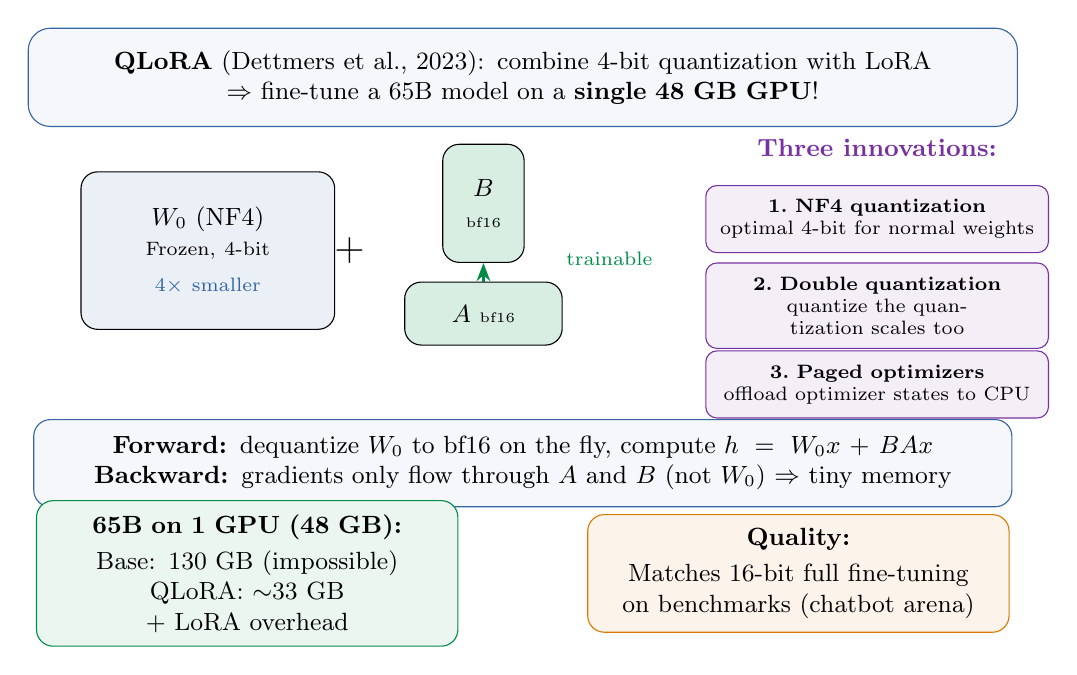
\begin{tikzpicture}
  % Idea
  \node[draw=popblue, fill=popblue!5, rounded corners=8pt, text width=12cm, align=center, inner sep=8pt, font=\small] at (0, 3.2) {
    \textbf{QLoRA} (Dettmers et al., 2023): combine 4-bit quantization with LoRA\\
    $\Rightarrow$ fine-tune a 65B model on a \textbf{single 48 GB GPU}!
  };

  % Architecture
  % Frozen quantized weights
  \node[draw, rounded corners=6pt, fill=popblue!10, minimum width=3cm, minimum height=2cm, text width=2.8cm, align=center, inner sep=6pt, font=\small] (W) at (-4, 1) {
    $W_0$ (NF4)\\{\scriptsize Frozen, 4-bit}\\[2pt]
    {\scriptsize \textcolor{popblue}{4$\times$ smaller}}
  };

  % LoRA in bf16
  \node[draw, rounded corners=6pt, fill=paramgreen!15, minimum width=1cm, minimum height=1.5cm, font=\small, text width=0.8cm, align=center] (B) at (-0.5, 1.6) {$B$\\{\tiny bf16}};
  \node[draw, rounded corners=6pt, fill=paramgreen!15, minimum width=2cm, minimum height=0.8cm, font=\small, text width=1.6cm, align=center] (A) at (-0.5, 0.2) {$A$ {\tiny bf16}};
  \draw[-Stealth, thick, paramgreen] (A) -- (B);
  \node[font=\scriptsize, text=paramgreen] at (1.1, 0.9) {trainable};

  \node[font=\Large] at (-2.2, 1) {$+$};

  % Three innovations
  \node[font=\small\bfseries, text=violet1] at (4.5, 2.3) {Three innovations:};

  \node[draw=violet1, fill=violet1!8, rounded corners=4pt, text width=4cm, align=center, inner sep=5pt, font=\scriptsize] at (4.5, 1.4) {
    \textbf{1.\ NF4 quantization}\\optimal 4-bit for normal weights
  };
  \node[draw=violet1, fill=violet1!8, rounded corners=4pt, text width=4cm, align=center, inner sep=5pt, font=\scriptsize] at (4.5, 0.3) {
    \textbf{2.\ Double quantization}\\quantize the quantization scales too
  };
  \node[draw=violet1, fill=violet1!8, rounded corners=4pt, text width=4cm, align=center, inner sep=5pt, font=\scriptsize] at (4.5, -0.7) {
    \textbf{3.\ Paged optimizers}\\offload optimizer states to CPU
  };

  % Forward pass
  \node[draw=popblue, fill=popblue!5, rounded corners=6pt, inner sep=6pt, text width=12cm, align=center, font=\small] at (0, -1.7) {
    \textbf{Forward:} dequantize $W_0$ to bf16 on the fly, compute $h = W_0 x + BAx$\\
    \textbf{Backward:} gradients only flow through $A$ and $B$ (not $W_0$) $\Rightarrow$ tiny memory
  };

  % Results
  \node[draw=paramgreen, fill=paramgreen!8, rounded corners=6pt, text width=5cm, align=center, inner sep=5pt, font=\small] at (-3.5, -3.1) {
    \textbf{65B on 1 GPU (48 GB):}\\[2pt]
    Base: 130 GB (impossible)\\QLoRA: $\sim$33 GB + LoRA overhead
  };
  \node[draw=orange1, fill=orange1!8, rounded corners=6pt, text width=5cm, align=center, inner sep=5pt, font=\small] at (3.5, -3.1) {
    \textbf{Quality:}\\[2pt]
    Matches 16-bit full fine-tuning\\on benchmarks (chatbot arena)
  };
\end{tikzpicture}
\end{center}
\end{frame}

% ============================================================
% PART III HEADER
% ============================================================
\begin{frame}
\begin{center}
\vspace{1.5cm}
{\Huge \textcolor{paramgreen}{Part III}}

\vspace{0.5cm}
{\Large Knowledge Distillation}

\vspace{0.5cm}
{\normalsize Training a small model to mimic a large one}
\end{center}
\end{frame}

% ============================================================
% KNOWLEDGE DISTILLATION
% ============================================================
\begin{frame}
\frametitle{Knowledge distillation --- teacher and student}

\begin{center}
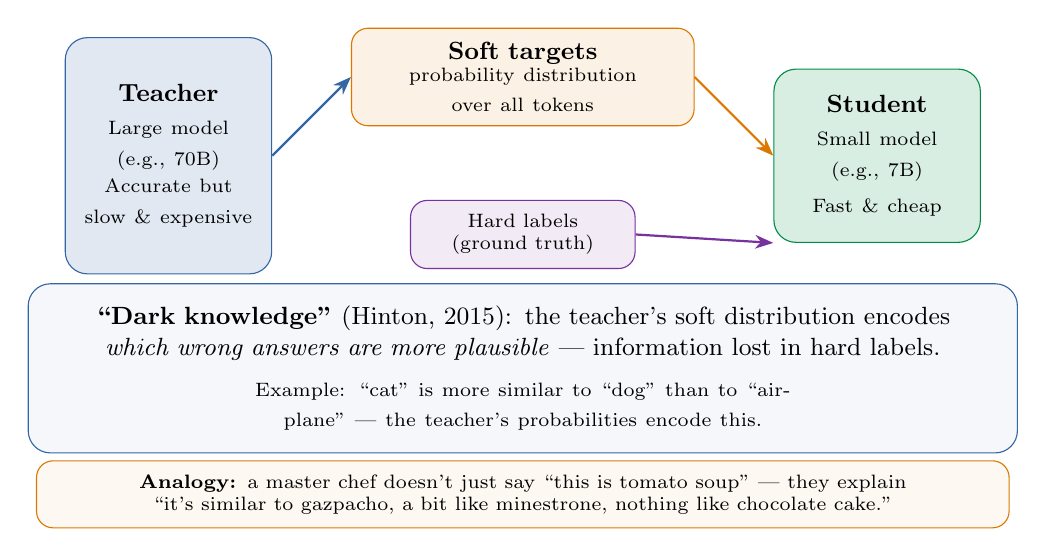
\begin{tikzpicture}
  % Teacher
  \node[draw=popblue, fill=popblue!15, rounded corners=8pt, minimum width=2.5cm, minimum height=3cm, text width=2.2cm, align=center, inner sep=6pt, font=\small] (teacher) at (-4.5, 1.5) {
    \textbf{Teacher}\\[4pt]
    {\scriptsize Large model\\(e.g., 70B)}\\[2pt]
    {\scriptsize Accurate but\\slow \& expensive}
  };

  % Student
  \node[draw=paramgreen, fill=paramgreen!15, rounded corners=8pt, minimum width=2.5cm, minimum height=2.2cm, text width=2.2cm, align=center, inner sep=6pt, font=\small] (student) at (4.5, 1.5) {
    \textbf{Student}\\[4pt]
    {\scriptsize Small model\\(e.g., 7B)}\\[2pt]
    {\scriptsize Fast \& cheap}
  };

  % Soft targets
  \node[draw=orange1, fill=orange1!10, rounded corners=6pt, text width=4cm, align=center, inner sep=5pt, font=\small] (soft) at (0, 2.5) {
    \textbf{Soft targets}\\{\scriptsize probability distribution\\over all tokens}
  };
  \draw[-Stealth, thick, popblue] (teacher.east) -- (soft.west);
  \draw[-Stealth, thick, orange1] (soft.east) -- (student.west);

  % Hard labels
  \node[draw=violet1, fill=violet1!10, rounded corners=6pt, text width=2.5cm, align=center, inner sep=5pt, font=\scriptsize] (hard) at (0, 0.5) {
    Hard labels\\(ground truth)
  };
  \draw[-Stealth, thick, violet1] (hard.east) -- (student.south west);

  % Dark knowledge explanation
  \node[draw=popblue, fill=popblue!5, rounded corners=8pt, text width=12cm, align=center, inner sep=8pt, font=\small] at (0, -1.2) {
    \textbf{``Dark knowledge''} (Hinton, 2015): the teacher's soft distribution encodes\\
    \emph{which wrong answers are more plausible} --- information lost in hard labels.\\[4pt]
    {\scriptsize Example: ``cat'' is more similar to ``dog'' than to ``airplane'' --- the teacher's probabilities encode this.}
  };

  % Analogy
  \node[draw=orange1, fill=orange1!5, rounded corners=6pt, text width=12cm, align=center, inner sep=5pt, font=\scriptsize] at (0, -2.8) {
    \textbf{Analogy:} a master chef doesn't just say ``this is tomato soup'' --- they explain\\``it's similar to gazpacho, a bit like minestrone, nothing like chocolate cake.''
  };
\end{tikzpicture}
\end{center}
\end{frame}

% ============================================================
% DISTILLATION LOSS
% ============================================================
\begin{frame}
\frametitle{The distillation loss}

\vspace{-0.2cm}
\begin{center}
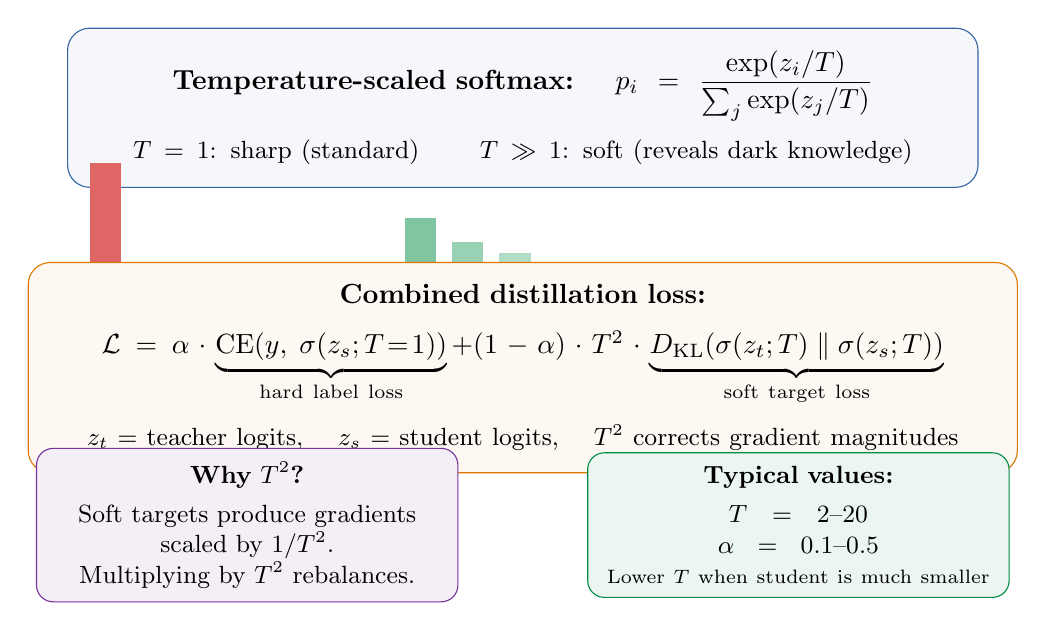
\begin{tikzpicture}
  % Temperature
  \node[draw=popblue, fill=popblue!5, rounded corners=8pt, inner sep=8pt, text width=11cm, align=center] at (0, 3) {
    \textbf{Temperature-scaled softmax:} \quad $\displaystyle p_i = \frac{\exp(z_i / T)}{\sum_j \exp(z_j / T)}$\\[6pt]
    {\small $T = 1$: sharp (standard) \qquad $T \gg 1$: soft (reveals dark knowledge)}
  };

  % Temperature visualization
  \fill[sampred!60] (-5.5, 0.8) rectangle (-5.1, 2.3);
  \fill[sampred!20] (-4.9, 0.8) rectangle (-4.5, 0.95);
  \fill[sampred!20] (-4.3, 0.8) rectangle (-3.9, 0.9);
  \fill[sampred!20] (-3.7, 0.8) rectangle (-3.3, 0.85);
  \node[font=\tiny] at (-4.4, 0.6) {$T=1$ (sharp)};

  \fill[paramgreen!50] (-1.5, 0.8) rectangle (-1.1, 1.6);
  \fill[paramgreen!40] (-0.9, 0.8) rectangle (-0.5, 1.3);
  \fill[paramgreen!30] (-0.3, 0.8) rectangle (0.1, 1.15);
  \fill[paramgreen!20] (0.3, 0.8) rectangle (0.7, 1.0);
  \node[font=\tiny] at (-0.4, 0.6) {$T=5$ (soft)};

  % Combined loss
  \node[draw=orange1, fill=orange1!5, rounded corners=8pt, inner sep=8pt, text width=12cm, align=center] at (0, -0.3) {
    \textbf{Combined distillation loss:}\\[6pt]
    {\normalsize $\mathcal{L} = \alpha \cdot \underbrace{\text{CE}\!\left(y,\; \sigma(z_s; T\!=\!1)\right)}_{\text{hard label loss}} + (1-\alpha) \cdot T^2 \cdot \underbrace{D_{\text{KL}}\!\left(\sigma(z_t; T) \;\|\; \sigma(z_s; T)\right)}_{\text{soft target loss}}$}\\[6pt]
    {\small $z_t$ = teacher logits, \quad $z_s$ = student logits, \quad $T^2$ corrects gradient magnitudes}
  };

  % Why T^2
  \node[draw=violet1, fill=violet1!8, rounded corners=6pt, text width=5cm, align=center, inner sep=5pt, font=\small] at (-3.5, -2.3) {
    \textbf{Why $T^2$?}\\[3pt]
    Soft targets produce gradients\\scaled by $1/T^2$.\\Multiplying by $T^2$ rebalances.
  };

  % Typical values
  \node[draw=paramgreen, fill=paramgreen!8, rounded corners=6pt, text width=5cm, align=center, inner sep=5pt, font=\small] at (3.5, -2.3) {
    \textbf{Typical values:}\\[3pt]
    $T = 2$--$20$\\$\alpha = 0.1$--$0.5$\\{\scriptsize Lower $T$ when student is much smaller}
  };
\end{tikzpicture}
\end{center}
\end{frame}

% ============================================================
% NOTABLE DISTILLED MODELS
% ============================================================
\begin{frame}
\frametitle{Notable distilled models}

\vspace{-0.2cm}
\renewcommand{\arraystretch}{1.4}
\begin{center}
{\small
\begin{tabular}{>{\bfseries}l l l c l}
  \textbf{Student} & \textbf{Teacher} & \textbf{Compression} & \textbf{Quality} & \textbf{Method} \\
  \hline
  \textcolor{popblue}{DistilBERT} & BERT (110M) & 1.7$\times$ (66M) & 97\% GLUE & KD + cosine loss \\[2pt]
  \textcolor{paramgreen}{TinyLlama} & LLaMA (7B) & 6.4$\times$ (1.1B) & Competitive & Pre-train 3T tokens \\[2pt]
  \textcolor{orange1}{Minitron 4B} & LLaMA 3.1 (8B) & 2$\times$ (4B) & +16\% vs scratch & Prune + distill \\[2pt]
  \textcolor{violet1}{DeepSeek-R1 7B} & R1 (671B MoE) & 96$\times$ & Beats 32B & 800k reasoning samples \\[2pt]
  \textcolor{sampred}{Llama 3.1 8B} & Llama 405B & 50$\times$ & $\approx$ teacher & Synthetic data KD \\
  \hline
\end{tabular}
}
\end{center}

\vspace{0.2cm}
\begin{center}
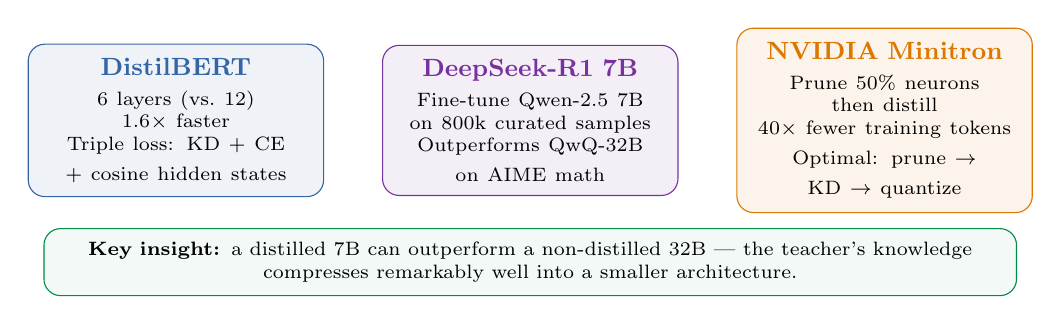
\begin{tikzpicture}
  % DistilBERT detail
  \node[draw=popblue, fill=popblue!8, rounded corners=6pt, text width=3.4cm, align=center, inner sep=5pt, font=\small] at (-4.5, 0) {
    \textbf{\textcolor{popblue}{DistilBERT}}\\[3pt]
    {\scriptsize 6 layers (vs.\ 12)\\1.6$\times$ faster\\Triple loss: KD + CE\\+ cosine hidden states}
  };

  % DeepSeek-R1 detail
  \node[draw=violet1, fill=violet1!8, rounded corners=6pt, text width=3.4cm, align=center, inner sep=5pt, font=\small] at (0, 0) {
    \textbf{\textcolor{violet1}{DeepSeek-R1 7B}}\\[3pt]
    {\scriptsize Fine-tune Qwen-2.5 7B\\on 800k curated samples\\Outperforms QwQ-32B\\on AIME math}
  };

  % Minitron
  \node[draw=orange1, fill=orange1!8, rounded corners=6pt, text width=3.4cm, align=center, inner sep=5pt, font=\small] at (4.5, 0) {
    \textbf{\textcolor{orange1}{NVIDIA Minitron}}\\[3pt]
    {\scriptsize Prune 50\% neurons\\then distill\\40$\times$ fewer training tokens\\Optimal: prune $\to$ KD $\to$ quantize}
  };

  % Key insight
  \node[draw=paramgreen, fill=paramgreen!5, rounded corners=6pt, text width=12cm, align=center, inner sep=5pt, font=\scriptsize] at (0, -1.8) {
    \textbf{Key insight:} a distilled 7B can outperform a non-distilled 32B --- the teacher's knowledge\\
    compresses remarkably well into a smaller architecture.
  };
\end{tikzpicture}
\end{center}
\end{frame}

% ============================================================
% PART IV HEADER
% ============================================================
\begin{frame}
\begin{center}
\vspace{1.5cm}
{\Huge \textcolor{violet1}{Part IV}}

\vspace{0.5cm}
{\Large Speculative Decoding}

\vspace{0.5cm}
{\normalsize Lossless acceleration via draft-then-verify}
\end{center}
\end{frame}

% ============================================================
% SPECULATIVE DECODING: CONCEPT
% ============================================================
\begin{frame}
\frametitle{Speculative decoding --- the idea}

\begin{center}
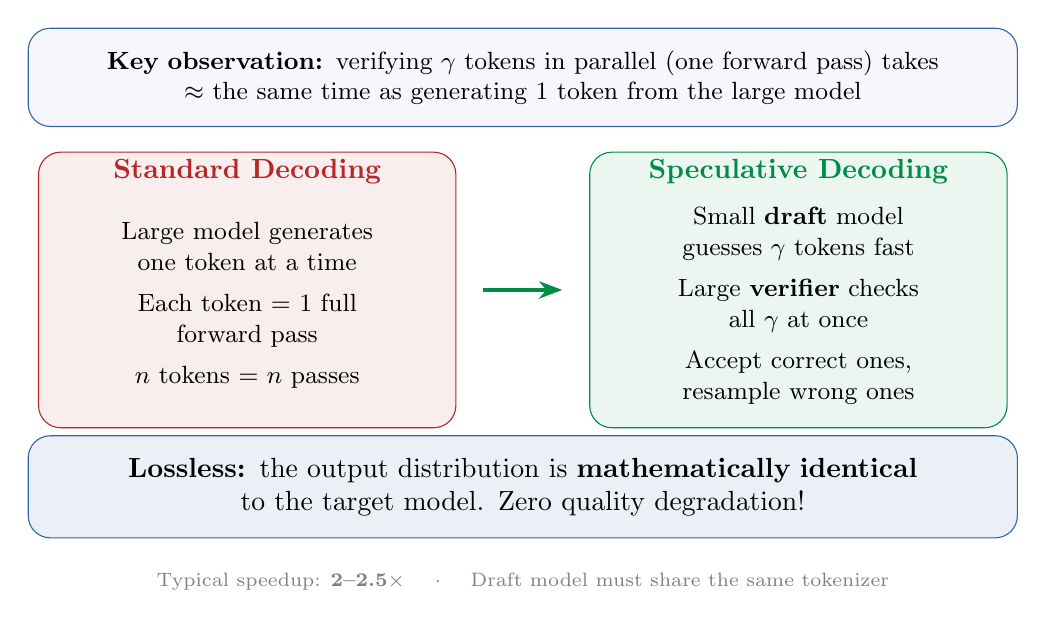
\begin{tikzpicture}
  % Key insight
  \node[draw=popblue, fill=popblue!5, rounded corners=8pt, text width=12cm, align=center, inner sep=8pt, font=\small] at (0, 3.2) {
    \textbf{Key observation:} verifying $\gamma$ tokens in parallel (one forward pass) takes\\
    $\approx$ the same time as generating 1 token from the large model
  };

  % Standard decoding
  \node[draw=warnred, fill=warnred!8, rounded corners=8pt, minimum width=5.3cm, minimum height=3.5cm, text width=4.8cm, align=center, inner sep=6pt] at (-3.5, 0.5) {};
  \node[font=\normalsize\bfseries, text=warnred] at (-3.5, 2) {Standard Decoding};
  \node[font=\small, text width=4.5cm, align=center] at (-3.5, 0.3) {
    Large model generates\\one token at a time\\[4pt]
    Each token = 1 full\\forward pass\\[4pt]
    $n$ tokens = $n$ passes
  };

  % Speculative decoding
  \node[draw=paramgreen, fill=paramgreen!8, rounded corners=8pt, minimum width=5.3cm, minimum height=3.5cm, text width=4.8cm, align=center, inner sep=6pt] at (3.5, 0.5) {};
  \node[font=\normalsize\bfseries, text=paramgreen] at (3.5, 2) {Speculative Decoding};
  \node[font=\small, text width=4.5cm, align=center] at (3.5, 0.3) {
    Small \textbf{draft} model\\guesses $\gamma$ tokens fast\\[4pt]
    Large \textbf{verifier} checks\\all $\gamma$ at once\\[4pt]
    Accept correct ones,\\resample wrong ones
  };

  \draw[-Stealth, very thick, paramgreen] (-0.5, 0.5) -- (0.5, 0.5);

  % Critical property
  \node[draw=popblue, fill=popblue!10, rounded corners=8pt, text width=12cm, align=center, inner sep=8pt, font=\normalsize] at (0, -2) {
    \textbf{Lossless:} the output distribution is \textbf{mathematically identical}\\
    to the target model. Zero quality degradation!
  };

  \node[font=\scriptsize, text=gray] at (0, -3.2) {
    Typical speedup: \textbf{2--2.5$\times$} \quad $\cdot$ \quad Draft model must share the same tokenizer
  };
\end{tikzpicture}
\end{center}
\end{frame}

% ============================================================
% SPECULATIVE DECODING: ALGORITHM
% ============================================================
\begin{frame}
\frametitle{Speculative decoding --- the algorithm}

\begin{center}
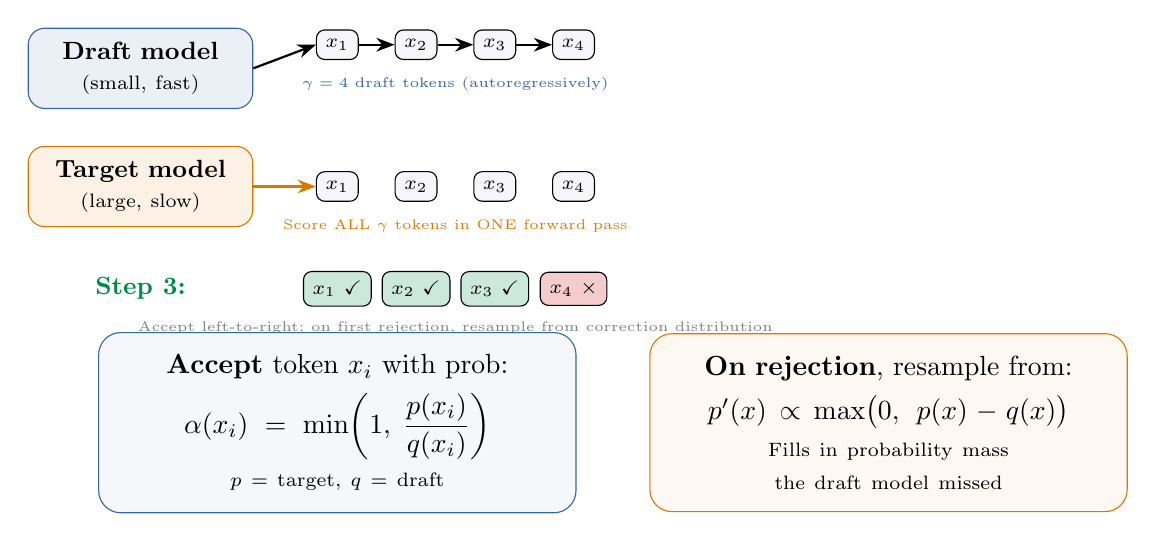
\begin{tikzpicture}
  % Step 1: Draft
  \node[draw=popblue, fill=popblue!10, rounded corners=6pt, text width=2.5cm, align=center, inner sep=5pt, font=\small] (draft) at (-5.5, 2.5) {
    \textbf{Draft model}\\{\scriptsize (small, fast)}
  };

  \node[draw, rounded corners=3pt, fill=lightbg, font=\scriptsize] (t1) at (-3, 2.8) {$x_1$};
  \node[draw, rounded corners=3pt, fill=lightbg, font=\scriptsize] (t2) at (-2, 2.8) {$x_2$};
  \node[draw, rounded corners=3pt, fill=lightbg, font=\scriptsize] (t3) at (-1, 2.8) {$x_3$};
  \node[draw, rounded corners=3pt, fill=lightbg, font=\scriptsize] (t4) at (0, 2.8) {$x_4$};
  \draw[-Stealth, thick] (draft.east) -- (t1.west);
  \draw[-Stealth, thick] (t1) -- (t2);
  \draw[-Stealth, thick] (t2) -- (t3);
  \draw[-Stealth, thick] (t3) -- (t4);
  \node[font=\tiny, text=popblue] at (-1.5, 2.3) {$\gamma = 4$ draft tokens (autoregressively)};

  % Step 2: Verify
  \node[draw=orange1, fill=orange1!10, rounded corners=6pt, text width=2.5cm, align=center, inner sep=5pt, font=\small] (verify) at (-5.5, 1) {
    \textbf{Target model}\\{\scriptsize (large, slow)}
  };

  \node[draw, rounded corners=3pt, fill=lightbg, font=\scriptsize] (v1) at (-3, 1) {$x_1$};
  \node[draw, rounded corners=3pt, fill=lightbg, font=\scriptsize] (v2) at (-2, 1) {$x_2$};
  \node[draw, rounded corners=3pt, fill=lightbg, font=\scriptsize] (v3) at (-1, 1) {$x_3$};
  \node[draw, rounded corners=3pt, fill=lightbg, font=\scriptsize] (v4) at (0, 1) {$x_4$};
  \draw[-Stealth, thick, orange1] (verify.east) -- (v1.west);
  \node[font=\tiny, text=orange1] at (-1.5, 0.5) {Score ALL $\gamma$ tokens in ONE forward pass};

  % Step 3: Accept/Reject
  \node[font=\small\bfseries, text=paramgreen] at (-5.5, -0.3) {Step 3:};
  \node[draw, rounded corners=3pt, fill=paramgreen!20, font=\scriptsize] at (-3, -0.3) {$x_1$ \checkmark};
  \node[draw, rounded corners=3pt, fill=paramgreen!20, font=\scriptsize] at (-2, -0.3) {$x_2$ \checkmark};
  \node[draw, rounded corners=3pt, fill=paramgreen!20, font=\scriptsize] at (-1, -0.3) {$x_3$ \checkmark};
  \node[draw, rounded corners=3pt, fill=sampred!20, font=\scriptsize] at (0, -0.3) {$x_4$ $\times$};

  \node[font=\tiny, text=gray] at (-1.5, -0.8) {Accept left-to-right; on first rejection, resample from correction distribution};

  % Acceptance criterion
  \node[draw=popblue, fill=popblue!5, rounded corners=8pt, inner sep=8pt, text width=5.5cm, align=center] at (-3, -2) {
    \textbf{Accept} token $x_i$ with prob:\\[4pt]
    {\normalsize $\alpha(x_i) = \min\!\left(1,\; \dfrac{p(x_i)}{q(x_i)}\right)$}\\[4pt]
    {\scriptsize $p$ = target, $q$ = draft}
  };

  % Correction distribution
  \node[draw=orange1, fill=orange1!5, rounded corners=8pt, inner sep=8pt, text width=5.5cm, align=center] at (4, -2) {
    \textbf{On rejection}, resample from:\\[4pt]
    {\normalsize $p'(x) \propto \max\!\big(0,\; p(x) - q(x)\big)$}\\[4pt]
    {\scriptsize Fills in probability mass\\the draft model missed}
  };
\end{tikzpicture}
\end{center}
\end{frame}

% ============================================================
% WHY LOSSLESS
% ============================================================
\begin{frame}
\frametitle{Why speculative decoding is lossless}

\begin{center}
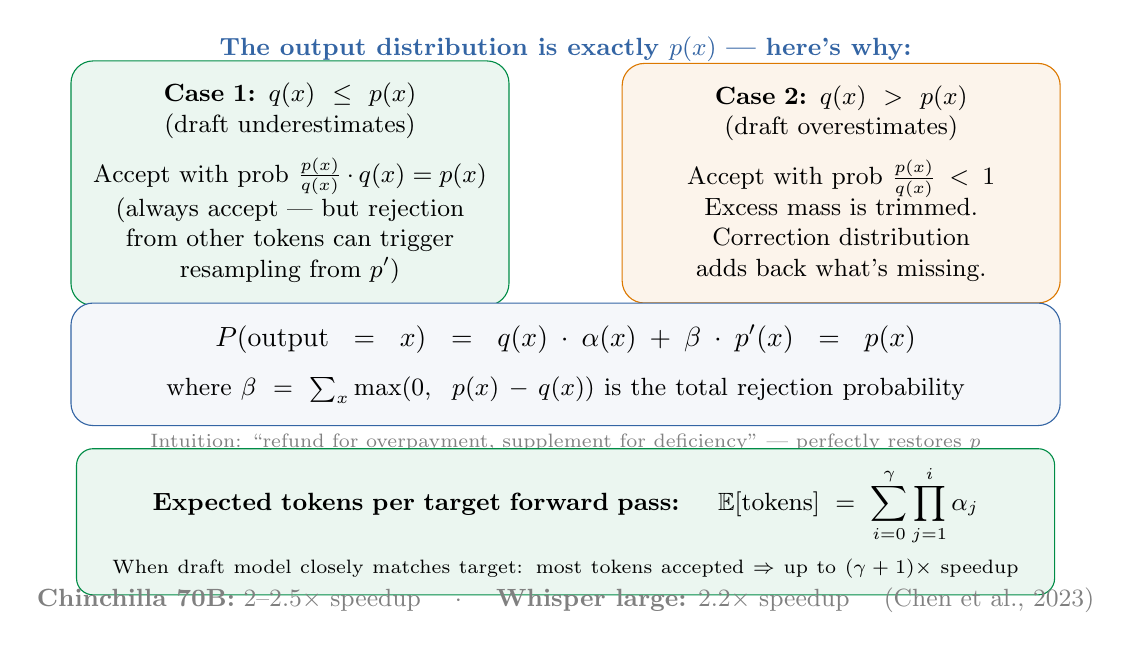
\begin{tikzpicture}
  % The proof idea
  \node[font=\small\bfseries, text=popblue] at (0, 3.5) {The output distribution is \textbf{exactly} $p(x)$ --- here's why:};

  % Two cases
  \node[draw=paramgreen, fill=paramgreen!8, rounded corners=8pt, text width=5cm, align=center, inner sep=8pt, font=\small] at (-3.5, 1.8) {
    \textbf{Case 1: $q(x) \leq p(x)$}\\(draft underestimates)\\[6pt]
    Accept with prob $\frac{p(x)}{q(x)} \cdot q(x) = p(x)$\\(always accept --- but rejection\\from other tokens can trigger\\resampling from $p'$)
  };

  \node[draw=orange1, fill=orange1!8, rounded corners=8pt, text width=5cm, align=center, inner sep=8pt, font=\small] at (3.5, 1.8) {
    \textbf{Case 2: $q(x) > p(x)$}\\(draft overestimates)\\[6pt]
    Accept with prob $\frac{p(x)}{q(x)} < 1$\\Excess mass is trimmed.\\Correction distribution\\adds back what's missing.
  };

  % Combined
  \node[draw=popblue, fill=popblue!5, rounded corners=8pt, inner sep=8pt, text width=12cm, align=center] at (0, -0.5) {
    {\normalsize $P(\text{output} = x) = q(x) \cdot \alpha(x) + \beta \cdot p'(x) = p(x)$}\\[6pt]
    {\small where $\beta = \sum_x \max(0,\; p(x) - q(x))$ is the total rejection probability}
  };

  \node[font=\scriptsize, text=gray] at (0, -1.5) {
    Intuition: ``refund for overpayment, supplement for deficiency'' --- perfectly restores $p$
  };

  % Expected tokens per step
  \node[draw=paramgreen, fill=paramgreen!8, rounded corners=6pt, text width=12cm, align=center, inner sep=6pt, font=\small] at (0, -2.5) {
    \textbf{Expected tokens per target forward pass:} \quad $\displaystyle \mathbb{E}[\text{tokens}] = \sum_{i=0}^{\gamma} \prod_{j=1}^{i} \alpha_j$\\[4pt]
    {\scriptsize When draft model closely matches target: most tokens accepted $\Rightarrow$ up to $(\gamma+1)\times$ speedup}
  };

  % Results
  \node[font=\small, text=gray] at (0, -3.5) {
    \textbf{Chinchilla 70B:} 2--2.5$\times$ speedup \quad $\cdot$ \quad \textbf{Whisper large:} 2.2$\times$ speedup \quad (Chen et al., 2023)
  };
\end{tikzpicture}
\end{center}
\end{frame}

% ============================================================
% SPECULATIVE DECODING: WORKED EXAMPLE
% ============================================================
\begin{frame}
\frametitle{Speculative decoding --- worked example}

\vspace{-0.2cm}
\begin{center}
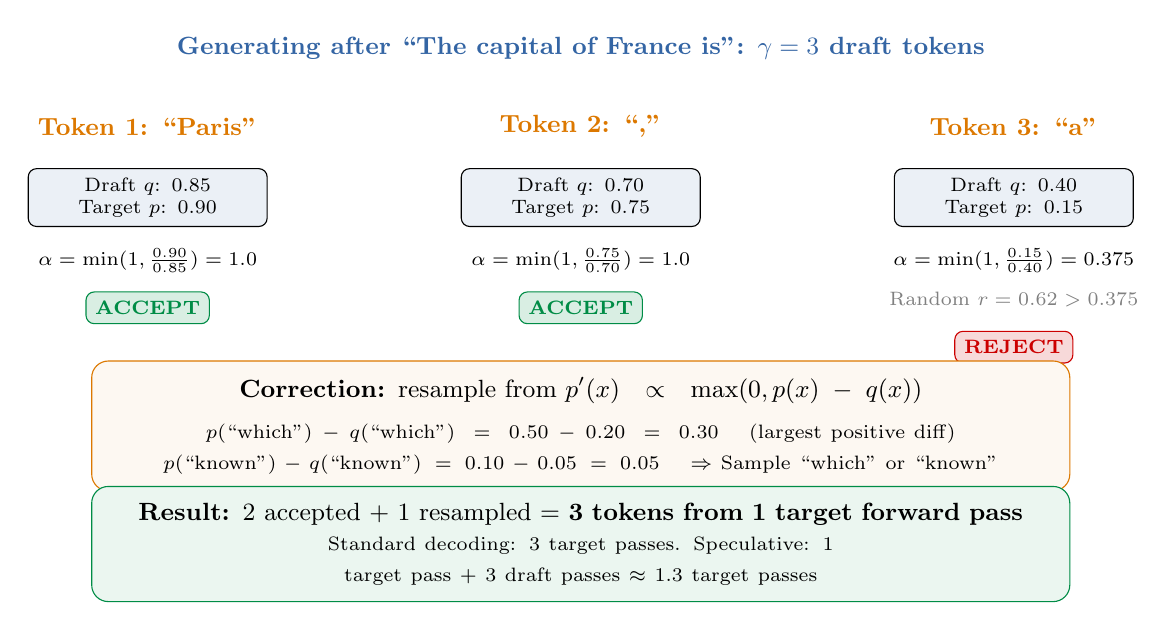
\begin{tikzpicture}
  \node[font=\small\bfseries, text=popblue] at (0, 3.5) {Generating after ``The capital of France is'': $\gamma = 3$ draft tokens};

  % Token: "Paris"
  \node[font=\small\bfseries, text=orange1] at (-5.5, 2.5) {Token 1: ``Paris''};

  \node[draw, rounded corners=3pt, fill=popblue!10, font=\scriptsize, text width=2.8cm, align=center] at (-5.5, 1.6) {
    Draft $q$: 0.85\\Target $p$: 0.90
  };
  \node[font=\scriptsize] at (-5.5, 0.8) {$\alpha = \min(1, \frac{0.90}{0.85}) = 1.0$};
  \node[draw=paramgreen, fill=paramgreen!15, rounded corners=3pt, font=\scriptsize\bfseries, text=paramgreen] at (-5.5, 0.2) {ACCEPT};

  % Token: ","
  \node[font=\small\bfseries, text=orange1] at (0, 2.5) {Token 2: ``,''};

  \node[draw, rounded corners=3pt, fill=popblue!10, font=\scriptsize, text width=2.8cm, align=center] at (0, 1.6) {
    Draft $q$: 0.70\\Target $p$: 0.75
  };
  \node[font=\scriptsize] at (0, 0.8) {$\alpha = \min(1, \frac{0.75}{0.70}) = 1.0$};
  \node[draw=paramgreen, fill=paramgreen!15, rounded corners=3pt, font=\scriptsize\bfseries, text=paramgreen] at (0, 0.2) {ACCEPT};

  % Token: "a" (rejected)
  \node[font=\small\bfseries, text=orange1] at (5.5, 2.5) {Token 3: ``a''};

  \node[draw, rounded corners=3pt, fill=popblue!10, font=\scriptsize, text width=2.8cm, align=center] at (5.5, 1.6) {
    Draft $q$: 0.40\\Target $p$: 0.15
  };
  \node[font=\scriptsize] at (5.5, 0.8) {$\alpha = \min(1, \frac{0.15}{0.40}) = 0.375$};
  \node[font=\scriptsize, text=gray] at (5.5, 0.3) {Random $r = 0.62 > 0.375$};
  \node[draw=sampred, fill=sampred!15, rounded corners=3pt, font=\scriptsize\bfseries, text=sampred] at (5.5, -0.3) {REJECT};

  % Correction
  \node[draw=orange1, fill=orange1!5, rounded corners=6pt, text width=12cm, align=center, inner sep=6pt, font=\small] at (0, -1.3) {
    \textbf{Correction:} resample from $p'(x) \propto \max(0, p(x) - q(x))$\\[4pt]
    {\scriptsize $p(\text{``which''}) - q(\text{``which''}) = 0.50 - 0.20 = 0.30$ \quad (largest positive diff)}\\
    {\scriptsize $p(\text{``known''}) - q(\text{``known''}) = 0.10 - 0.05 = 0.05$ \quad $\Rightarrow$ Sample ``which'' or ``known''}
  };

  % Result
  \node[draw=paramgreen, fill=paramgreen!8, rounded corners=6pt, text width=12cm, align=center, inner sep=6pt, font=\small] at (0, -2.8) {
    \textbf{Result:} 2 accepted + 1 resampled $=$ \textbf{3 tokens from 1 target forward pass}\\
    {\scriptsize Standard decoding: 3 target passes. Speculative: 1 target pass + 3 draft passes $\approx$ 1.3 target passes}
  };
\end{tikzpicture}
\end{center}
\end{frame}

% ============================================================
% CONTINUOUS BATCHING & vLLM
% ============================================================
\begin{frame}
\frametitle{Production serving: continuous batching}

\begin{center}
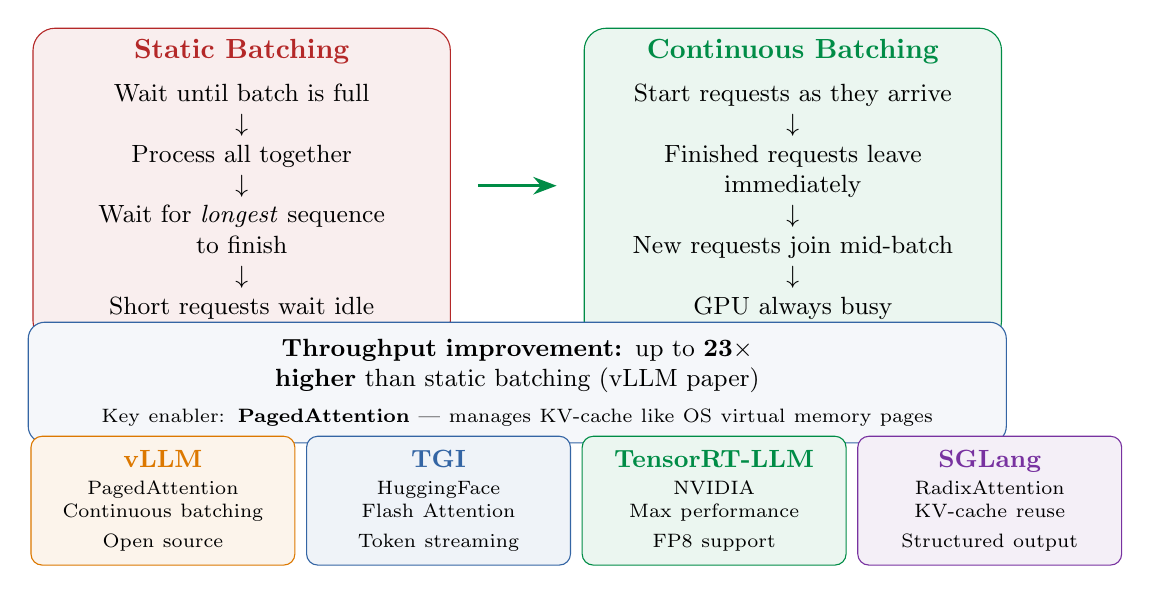
\begin{tikzpicture}
  % Static batching problem
  \node[draw=warnred, fill=warnred!8, rounded corners=8pt, minimum width=5.3cm, minimum height=4cm, text width=4.8cm, align=center, inner sep=6pt] at (-3.5, 1) {};
  \node[font=\normalsize\bfseries, text=warnred] at (-3.5, 2.7) {Static Batching};

  \node[font=\small, text width=4.5cm, align=center] at (-3.5, 0.8) {
    Wait until batch is full\\$\downarrow$\\Process all together\\$\downarrow$\\Wait for \emph{longest} sequence\\to finish\\$\downarrow$\\Short requests wait idle
  };

  % Continuous batching
  \node[draw=paramgreen, fill=paramgreen!8, rounded corners=8pt, minimum width=5.3cm, minimum height=4cm, text width=4.8cm, align=center, inner sep=6pt] at (3.5, 1) {};
  \node[font=\normalsize\bfseries, text=paramgreen] at (3.5, 2.7) {Continuous Batching};

  \node[font=\small, text width=4.5cm, align=center] at (3.5, 0.8) {
    Start requests as they arrive\\$\downarrow$\\Finished requests leave\\immediately\\$\downarrow$\\New requests join mid-batch\\$\downarrow$\\GPU always busy
  };

  \draw[-Stealth, very thick, paramgreen] (-0.5, 1) -- (0.5, 1);

  % Throughput improvement
  \node[draw=popblue, fill=popblue!5, rounded corners=6pt, text width=12cm, align=center, inner sep=6pt, font=\small] at (0, -1.5) {
    \textbf{Throughput improvement:} up to \textbf{23$\times$ higher} than static batching (vLLM paper)\\[2pt]
    {\scriptsize Key enabler: \textbf{PagedAttention} --- manages KV-cache like OS virtual memory pages}
  };

  % Tools
  \node[draw=orange1, fill=orange1!8, rounded corners=4pt, text width=3cm, align=center, inner sep=5pt, font=\small] at (-4.5, -3) {
    \textbf{\textcolor{orange1}{vLLM}}\\[2pt]
    {\scriptsize PagedAttention\\Continuous batching\\Open source}
  };
  \node[draw=popblue, fill=popblue!8, rounded corners=4pt, text width=3cm, align=center, inner sep=5pt, font=\small] at (-1, -3) {
    \textbf{\textcolor{popblue}{TGI}}\\[2pt]
    {\scriptsize HuggingFace\\Flash Attention\\Token streaming}
  };
  \node[draw=paramgreen, fill=paramgreen!8, rounded corners=4pt, text width=3cm, align=center, inner sep=5pt, font=\small] at (2.5, -3) {
    \textbf{\textcolor{paramgreen}{TensorRT-LLM}}\\[2pt]
    {\scriptsize NVIDIA\\Max performance\\FP8 support}
  };
  \node[draw=violet1, fill=violet1!8, rounded corners=4pt, text width=3cm, align=center, inner sep=5pt, font=\small] at (6, -3) {
    \textbf{\textcolor{violet1}{SGLang}}\\[2pt]
    {\scriptsize RadixAttention\\KV-cache reuse\\Structured output}
  };
\end{tikzpicture}
\end{center}
\end{frame}

% ============================================================
% ALL TECHNIQUES COMPARED
% ============================================================
\begin{frame}
\frametitle{Inference optimization techniques compared}

\vspace{-0.2cm}
\renewcommand{\arraystretch}{1.4}
\begin{center}
{\scriptsize
\begin{tabular}{>{\bfseries}l l l l l}
  \textbf{Technique} & \textbf{What it does} & \textbf{Memory} & \textbf{Speed} & \textbf{Quality} \\
  \hline
  \textcolor{popblue}{KV-Cache} & Cache K, V across steps & $\uparrow$ (linear in seq) & $\sim$5$\times$ $\uparrow$ & Identical \\[2pt]
  \textcolor{popblue}{MQA/GQA} & Share K/V heads & KV-cache $\downarrow\downarrow$ & Faster & Near-identical \\[2pt]
  \textcolor{popblue}{Flash Attn} & Tile attention in SRAM & $O(N)$ vs $O(N^2)$ & Faster & Identical \\[2pt]
  \textcolor{orange1}{Quantization} & Lower bit precision & 50--75\% $\downarrow$ & Depends & $\sim$2--3\% $\downarrow$ \\[2pt]
  \textcolor{paramgreen}{Distillation} & Train smaller model & Model size $\downarrow\downarrow$ & Much faster & 3--10\% $\downarrow$ \\[2pt]
  \textcolor{violet1}{Spec.\ Decoding} & Draft + verify & Slight $\uparrow$ & 2--2.5$\times$ $\uparrow$ & Identical \\
  \hline
\end{tabular}
}
\end{center}

\vspace{0.3cm}
\begin{center}
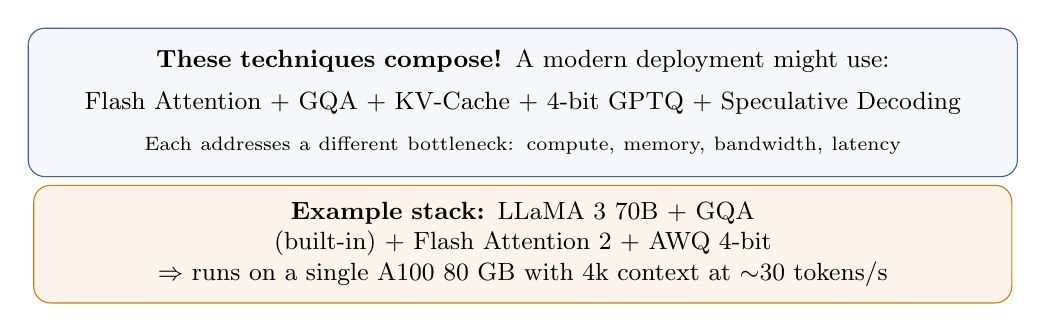
\begin{tikzpicture}
  % Composability note
  \node[draw=popblue, fill=popblue!5, rounded corners=6pt, text width=12cm, align=center, inner sep=8pt, font=\small] at (0, 0.3) {
    \textbf{These techniques compose!} A modern deployment might use:\\[4pt]
    Flash Attention + GQA + KV-Cache + 4-bit GPTQ + Speculative Decoding\\[4pt]
    {\scriptsize Each addresses a different bottleneck: compute, memory, bandwidth, latency}
  };

  % Production stack example
  \node[draw=orange1, fill=orange1!8, rounded corners=6pt, text width=12cm, align=center, inner sep=6pt, font=\small] at (0, -1.5) {
    \textbf{Example stack:} LLaMA 3 70B + GQA (built-in) + Flash Attention 2 + AWQ 4-bit\\
    $\Rightarrow$ runs on a single A100 80 GB with 4k context at $\sim$30 tokens/s
  };
\end{tikzpicture}
\end{center}
\end{frame}

% ============================================================
% PRACTICAL GUIDE
% ============================================================
\begin{frame}
\frametitle{Practical guide}

\begin{center}
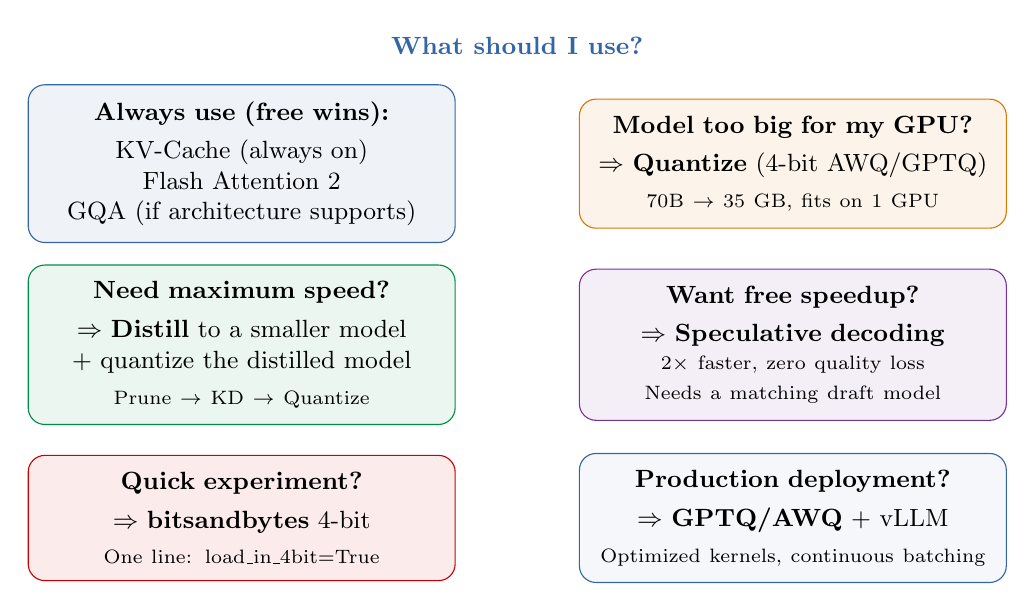
\begin{tikzpicture}
  \node[font=\small\bfseries, text=popblue] at (0, 3.5) {What should I use?};

  % Decision boxes
  \node[draw=popblue, fill=popblue!8, rounded corners=6pt, text width=5cm, align=center, inner sep=6pt, font=\small] at (-3.5, 2) {
    \textbf{Always use (free wins):}\\[3pt]
    KV-Cache (always on)\\Flash Attention 2\\GQA (if architecture supports)
  };
  \node[draw=orange1, fill=orange1!8, rounded corners=6pt, text width=5cm, align=center, inner sep=6pt, font=\small] at (3.5, 2) {
    \textbf{Model too big for my GPU?}\\[3pt]
    $\Rightarrow$ \textbf{Quantize} (4-bit AWQ/GPTQ)\\[2pt]
    {\scriptsize 70B $\to$ 35 GB, fits on 1 GPU}
  };
  \node[draw=paramgreen, fill=paramgreen!8, rounded corners=6pt, text width=5cm, align=center, inner sep=6pt, font=\small] at (-3.5, -0.3) {
    \textbf{Need maximum speed?}\\[3pt]
    $\Rightarrow$ \textbf{Distill} to a smaller model\\+ quantize the distilled model\\[2pt]
    {\scriptsize Prune $\to$ KD $\to$ Quantize}
  };
  \node[draw=violet1, fill=violet1!8, rounded corners=6pt, text width=5cm, align=center, inner sep=6pt, font=\small] at (3.5, -0.3) {
    \textbf{Want free speedup?}\\[3pt]
    $\Rightarrow$ \textbf{Speculative decoding}\\[2pt]
    {\scriptsize 2$\times$ faster, zero quality loss\\Needs a matching draft model}
  };
  \node[draw=sampred, fill=sampred!8, rounded corners=6pt, text width=5cm, align=center, inner sep=6pt, font=\small] at (-3.5, -2.5) {
    \textbf{Quick experiment?}\\[3pt]
    $\Rightarrow$ \textbf{bitsandbytes} 4-bit\\[2pt]
    {\scriptsize One line: load\_in\_4bit=True}
  };
  \node[draw=popblue, fill=popblue!5, rounded corners=6pt, text width=5cm, align=center, inner sep=6pt, font=\small] at (3.5, -2.5) {
    \textbf{Production deployment?}\\[3pt]
    $\Rightarrow$ \textbf{GPTQ/AWQ} + vLLM\\[2pt]
    {\scriptsize Optimized kernels, continuous batching}
  };
\end{tikzpicture}
\end{center}
\end{frame}

% ============================================================
% QUESTIONS
% ============================================================
\begin{frame}
\begin{center}
\vspace{2cm}
{\Huge \textcolor{popblue}{Questions?}}

\vspace{1cm}
{\large Next: RAG --- Retrieval-Augmented Generation}
\end{center}
\end{frame}

\end{document}
